\documentclass{article}
\usepackage[T2A]{fontenc}
\usepackage[utf8]{inputenc}
\usepackage[russian]{babel}
\usepackage{amssymb}
\usepackage{mathtools}
\usepackage{hyperref}
\usepackage{xcolor}
\usepackage{relsize}
\usepackage{wrapfig}
\usepackage[left=2cm,right=2cm,top=2cm,bottom=2cm,bindingoffset=0cm]{geometry}

\addto\captionsrussian{
  \renewcommand{\contentsname}
    {\huge\centering{СОДЕРЖАНИЕ}}
}

\begin{document}
\textbf{\huge Алгебра, коллоквиум}
\Large
\newline $ $
\newline vk: \href{https://vk.com/uselessofflane}{\color{blue}vk.com/uselessofflane},\, tg: \href{https://t.me/fmakhnach}{\color{blue}@fmakhnach}
\newline Были использованы материалы \textbf{Sofiika}: \href{https://github.com/Sofiika/AlgebraKollok}{\color{blue} github.com/Sofiika/AlgebraKollok }

\tableofcontents

\newpage
\addcontentsline{toc}{section}{\LARGE \underline{ОПРЕДЕЛЕНИЯ} }
\section*{\LARGE\centering \underline{ОПРЕДЕЛЕНИЯ}}

\addcontentsline{toc}{section}{\Large \underline{Модуль 1} }
\section*{\LARGE\centering \underline{Модуль 1}}

\addcontentsline{toc}{subsection}{ 1.1. Дать определение умножения матриц. Коммутативна ли эта операция? Ответ пояснить. }
\section*{\LARGE \textbf{1.1. Дать определение умножения матриц. Коммутативна ли эта операция? Ответ пояснить.}}

Пусть даны две прямоугольных матрицы $A$ и $B$ размерности $n \times m$ и $m \times k$ соответственно. Произведением матриц $A$ и $B$ (обозначается как $A \times B$ или $AB$) называется такая матрица $C$ размерности $n \times k$, что её элементы задаются формулой 
$$
c_{ij} = \sum_{r = 1}^{m}(a_{ir}\cdot b_{rj}), \mbox{где }\; i = \overline{1, n};\, j = \overline{1, k}
$$
Умножение матриц возможно тогда и только тогда, когда количество столбцов первой матрицы равно количеству строк второй. Из этого следует некоммутитивность этой операции ($\exists A \times B \not\Rightarrow \exists B \times A$).

\addcontentsline{toc}{subsection}{ 1.2. Дать определения ступенчатого вида матрицы и канонического вида матрицы. }
\section*{\LARGE 1.2. Дать определения ступенчатого вида матрицы и канонического вида матрицы. }


Матрица $M$ имеет ступенчатый вид, если номера первых ненулевых элементов всех строк возрастают, а все нулевые строки находятся на нижних строках матрицы.
\newline Матрица $M$ имеет канонический (улучшенный ступенчатый) вид, если она имеет ступенчатый вид, а также все первые ненулевые (ведущие) элементы всех строк равны единице и являются единственными нунулевыми элементами в своих столбцах.

\addcontentsline{toc}{subsection}{ 1.3. Перечислить элементарные преобразования строк матрицы. }
\section*{\LARGE 1.3. Перечислить элементарные преобразования строк матрицы. }

1) умножение $i$-ой строки на число $\lambda \ne 0$;
\newline 2) перестановка местами двух строк;
\newline 3) добавление к $i$-ой строке $j$-ой строки с коэффициентом $\lambda \ne 0$.

\addcontentsline{toc}{subsection}{ 1.4. Сформулировать теорему о методе Гаусса.  }
\section*{\LARGE 1.4. Сформулировать теорему о методе Гаусса.  }

Любую конечную матрицу можно элементарными преобразованиями строк привести к каноническому виду.

\addcontentsline{toc}{subsection}{ 1.5. Дать определения перестановки и подстановки.  }
\section*{\LARGE 1.5. Дать определения перестановки и подстановки.  }

Перестановка -- упорядоченный набор чисел $1, 2 \,...\, n$ без повторений.
\newline Подстановка -- взаимнооднозначное отображение множества $\{1, 2 \,...\, n\}$ в самого себя, $n$ называется степенью подстановки.

\addcontentsline{toc}{subsection}{ 1.6. Выписать общую формулу для вычисления определителя произвольного порядка.  }
\section*{\LARGE 1.6. Выписать общую формулу для вычисления определителя произвольного порядка.  }

Пусть $\sigma(\varphi)$ -- число инверсий подстановки $\varphi$.
$$
\det{A} = \sum_{\varphi \in Sn}(-1)^{\sigma(\varphi)}a_{\varphi(1)1}\cdot...\cdot a_{\varphi(n)n} = \sum_{\varphi \in Sn}(-1)^{\sigma(\varphi)} \prod_{i = 1}^n a_{\varphi(i)i}
$$

\addcontentsline{toc}{subsection}{ 1.7. Что такое алгебраическое дополнение?  }
\section*{\LARGE 1.7. Что такое алгебраическое дополнение?  }

Алгебраическим дополнением элемента $a_{ij}$ матрицы $A$ называется число 
\newline $A_{ij} = (-1)^{i + j}\cdot M_{ij}$, где $M_{ij}$ -- дополнительный минор, т.е. определитель матрицы, получающейся из матрицы $A$ путём исключения $i$-ой строки и $j$-ого столбца.

\addcontentsline{toc}{subsection}{ 1.8. Выписать формулы для разложения определителя по строке и по столбцу. }
\section*{\LARGE 1.8. Выписать формулы для разложения определителя по строке и по столбцу. }

По $i$-ой строке:
$$
\det{A} = \sum_{j = 1}^n a_{ij}A_{ij}
$$
По $j$-ому столбцу:
$$
\det{A} = \sum_{i = 1}^n a_{ij}A_{ij}
$$

\addcontentsline{toc}{subsection}{ 1.9. Что такое фальшивое разложение?  }
\section*{\LARGE 1.9. Что такое фальшивое разложение?  }

Фальшивое разложение -- следствие из теоремы Лапласа, заключающееся в следующем: сумма произведений всех элементов некоторой строки (столбца) матрицы $A$ на алгебраические дополнения соответствующих элементов любой \underline{другой} строки (столбца) равна нулю.
$$
\sum_{i = 1}^n a_{ij_1}A_{ij_2} = \sum_{j = 1}^n a_{i_1j}A_{i_2j} = 0, \;\;\;i_1 \ne i_2, \; j_1 \ne j_2
$$

\addcontentsline{toc}{subsection}{ 1.10. Выписать формулы Крамера для квадратной матрицы произвольного порядка. Когда с их помощью можно найти решение СЛАУ?  }
\section*{\LARGE 1.10. Выписать формулы Крамера для квадратной матрицы произвольного порядка. Когда с их помощью можно найти решение СЛАУ?  }

Пусть есть столбец $b = \begin{pmatrix} b_1 \\ \vdots \\ b_n \end{pmatrix}$ и квадратная матрица $A$ размера $n \times n$
$$
A = 
\begin{pmatrix}
a_{11} & ... & a_{1n} \\
\vdots &  & \vdots \\
a_{n1} & ... & a_{nn} \\
\end{pmatrix}
$$
которые соответствуют СЛАУ
$$
\begin{cases}
a_{11}x_1 + ... + a_{1n}x_n = b_1 \\
... \\
a_{n1}x_1 + ... + a_{nn}x_n = b_n \\
\end{cases}
$$
Введём $\Delta_i$ как определитель матрицы, получающейся из $A$ заменой $i$-ого столбца на столбец $b$:
$$
\Delta_i = 
\begin{vmatrix}
a_{11} & ... & a_{1i-1} & b_1 & a_{1i+1} & ... & a_{1n} \\
... & ... & ... & ... & ... & ... & ... \\
a_{n1} & ... & a_{ni-1} & b_n & a_{ni+1} & ... & a_{nn} \\
\end{vmatrix}
$$
Тогда неизвествую $x_i \; (1 \le i \le n))$ можно найти по формуле
$$
x_i = \frac{\Delta_i}{\Delta}
$$
где $\Delta = \det{A}$.
\newline Найти решение СЛАУ этим методом можно тогда и только тогда, когда 
\newline $\det{A} \ne 0$.

\addcontentsline{toc}{subsection}{ 1.11. Дать определение союзной матрицы.  }
\section*{\LARGE 1.11. Дать определение союзной матрицы.  }

Матрица $C$ называется союзной относительно матрицы $A$, если она составлена из алгебраических дополнений соответствующих элементов транспонированной матрицы $A^T$:
$$
C = 
\begin{pmatrix}
A_{11} & ... & A_{n1} \\
... & ... & ... \\
A_{1n} & ... & A_{nn} \\
\end{pmatrix}
$$

\addcontentsline{toc}{subsection}{ 1.12. Дать определение обратной матрицы. Сформулировать критерий её существования. }
\section*{\LARGE 1.12. Дать определение обратной матрицы. Сформулировать критерий её существования. }

Матрица $A^{-1}$ называется обратной квадратной матрице $A$, если $A^{-1}A = AA^{-1} = E$ (единичная матрица). Обратная матрица для матрицы $A$ существует тогда и только тогда, когда $A$ -- квадратная и $\det{A} \ne 0$.

\addcontentsline{toc}{subsection}{ 1.13. Выписать формулу для нахождения обратной матрицы. }
\section*{\LARGE 1.13. Выписать формулу для нахождения обратной матрицы. }

$$
A^{-1} = \frac{1}{\det{A}}\cdot C
$$
где $C$ -- союзная к $A$ матрица, то есть 
$$
A^{-1} = \frac{1}{\det{A}}
\begin{pmatrix}
A_{11} & ... & A_{n1} \\
... & ... & ... \\
A_{1n} & ... & A_{nn} \\
\end{pmatrix}
$$

\addcontentsline{toc}{subsection}{ 1.14. Дать определение минора. }
\section*{\LARGE 1.14. Дать определение минора. }

Минором порядка $k$ матрицы $A$ называется определитель матрицы $k \times k$, состоящей из элементов, стоящих на пересечении заданных $k$ строк и $k$ столбцов матрицы $A$.
\newline Минором $M_{ij}$ зачастую обозначается минор, полученный исключением из исходной матрицы $i$-ой строки и $j$-ого столбца. 

\addcontentsline{toc}{subsection}{ 1.15. Дать определение базисного минора. Какие строки называются базисными?  }
\section*{\LARGE 1.15. Дать определение базисного минора. Какие строки называются базисными?  }

Базисным называется любой ненулевой минор матрицы максимального порядка. Порядок минора = порядок матрицы, определителем которой является минор.
\newline Строки, входящие в базисный минор называются базисными.

\addcontentsline{toc}{subsection}{ 1.16. Дать определение ранга матрицы.  }
\section*{\LARGE 1.16. Дать определение ранга матрицы.  }

Рангом матрицы называется наибольший порядок ненулевого минора матрицы.

\addcontentsline{toc}{subsection}{ 1.17. Дать определение линейной комбинации строк. Что такое нетривиальная линейная комбинация?  }
\section*{\LARGE 1.17. Дать определение линейной комбинации строк. Что такое нетривиальная линейная комбинация?  }

Линейной комбинацией строк $s_1, ..., s_k$ называется выражение $a_1s_1 + ... + a_ks_k$, где $a_1, ... , a_k$ -- произвольные коэффициенты.
\newline Линейная комбинация строк называется \underline{нетривиальной}, если $\exists a_i \ne 0$.

\addcontentsline{toc}{subsection}{ 1.18. Дать определение линейной зависимости строк матрицы.  }
\section*{\LARGE 1.18. Дать определение линейной зависимости строк матрицы.  }

Система строк матрицы называется линейно зависимой, если существует их нетривиальная линейная комбинация, равная нулевой строке.

\addcontentsline{toc}{subsection}{ 1.19. Дать определение линейно независимых столбцов матрицы.  }
\section*{\LARGE 1.19. Дать определение линейно независимых столбцов матрицы.  }

Система столбцов матрицы называется линейно независимой, если не существует их нетривиальной линейной комбинации, равной нулевому столбцу.

\addcontentsline{toc}{subsection}{ 1.20. Сформулировать критерий линейной зависимости.  }
\section*{\LARGE 1.20. Сформулировать критерий линейной зависимости.  }

Система строк линейно зависима тогда и только тогда, когда одна из строк может быть представлена как линейная комбинация оставшихся.

\addcontentsline{toc}{subsection}{ 1.21. Сформулировать теорему о базисном миноре.  }
\section*{\LARGE 1.21. Сформулировать теорему о базисном миноре.  }

Строки (столбцы) матрицы $A$, входящие в базисный минор, образуют линейно независимую систему. Любая строка (столбец) $A$ выражается через линейную комбинацию строк (столбцов) базисного минора.

\addcontentsline{toc}{subsection}{ 1.22. Сформулировать теорему о ранге матрицы.  }
\section*{\LARGE 1.22. Сформулировать теорему о ранге матрицы.  }

Ранг матрицы равен максимальному числу линейно независимых строк (столбцов) матрицы.

\addcontentsline{toc}{subsection}{ 1.23. Сформулировать критерий невырожденности квадратной матрицы. }
\section*{\LARGE 1.23. Сформулировать критерий невырожденности квадратной матрицы. }

Не знаю, что из этого критерий, а что определение, но для произвольной квадратной матрицы $A$ размера $n \times n$ следующие три условия эквивалентны:
\newline 1) $\det{A} \ne 0$
\newline 2) $RgA = n$
\newline 3) Все строки (столбцы) матрицы $A$ линейно независимы

\addcontentsline{toc}{subsection}{ 1.24. Выписать свойства решений однородных и неоднородных СЛАУ.  }
\section*{\LARGE 1.24. Выписать свойства решений однородных и неоднородных СЛАУ.  }

Однородная СЛАУ: $Ax = 0$
\newline Неоднородная СЛАУ: $Ax = b$
\newline $ $
\newline \underline{Однородные СЛАУ}:
\newline Если столбцы $x^1, ..., x^k$ -- решения однородной СЛАУ $Ax = 0$, то любая их линейная комбинация также является решением этой СЛАУ. Так, если однородная СЛАУ имеет ненулевое решение, она имеет бесконечно много решений.
\newline $ $
\newline \underline{Неоднородные СЛАУ}:
\newline Если $x^0$ -- решение $Ax = b$, то произвольный столбец $x$ является решением этой СЛАУ тогда и только тогда, когда $x = x^0 + y$, где $y$ -- решение соответствующей однородной СЛАУ, то есть $Ay = 0$.
\newline Если $x^1, x^2$ -- решения СЛАУ $Ax = b$, то $y = x^1 - x^2$ является решением однородной СЛАУ $Ax = 0$.

\addcontentsline{toc}{subsection}{ 1.25. Сформулировать теорему Кронекера–Капелли.  }
\section*{\LARGE 1.25. Сформулировать теорему Кронекера–Капелли.  }

СЛАУ $Ax = b$ совместна тогда и только тогда, когда $RgA = Rg[Ab]$, где $[Ab]$ -- матрица, полученная из столбцов матрицы $A$ и столбца $b$. 

\addcontentsline{toc}{subsection}{ 1.26. Дать определение фундаментальной системы решений (ФСР) однородной СЛАУ. }
\section*{\LARGE 1.26. Дать определение фундаментальной системы решений (ФСР) однородной СЛАУ. }

ФСР однородной СЛАУ $Ax = 0$ -- наибольшее возможное множество линейно независимых решений данной СЛАУ. Всего таких решений $n_x -  RgA$, где $n_x$ -- число переменных в СЛАУ.

\addcontentsline{toc}{subsection}{ 1.27. Сформулировать критерий существования ненулевого решения однородной системы линейных уравнений с квадратной матрицей.
 }
\section*{\LARGE 1.27. Сформулировать критерий существования ненулевого решения однородной системы линейных уравнений с квадратной матрицей. }

Однородная СЛАУ $Ax = 0$ с квадратной матрицей $A$ имеет ненулевое решение тогда и только тогда, когда $\det{A} = 0$, т.е. матрица вырождена.

\newpage
\addcontentsline{toc}{section}{\Large \underline{Модуль 2} }
\section*{\LARGE\centering \underline{Модуль 2}}

\addcontentsline{toc}{subsection}{ 2.1. Сформулируйте теорему о структуре общего решения однородной СЛАУ. }
\section*{\LARGE 2.1. Сформулируйте теорему о структуре общего решения однородной СЛАУ.  }

Пусть $f_1, f_2, ..., f_k$ ($k = n - r$) -- ФСР однородной СЛАУ $Ax = 0$. Тогда $x = \lambda_1f_1 + \lambda_2f_2 + ... + \lambda_kf_k$ является решением СЛАУ при любых $\lambda_1, ..., \lambda_k$. Иными словами, любое решение СЛАУ является линейной комбинацией ФСР.

\addcontentsline{toc}{subsection}{ 2.2. Сформулируйте теорему о структуре общего решения неоднородной системы линейных алгебраических уравнений.  }
\section*{\LARGE 2.2. Сформулируйте теорему о структуре общего решения неоднородной системы линейных алгебраических уравнений. }

Пусть $f_1, f_2, ..., f_k$ ($k = n - r$) -- ФСР однородной СЛАУ $Ax = 0$, а также известно некоторое частное решение $x_0$ неоднородной СЛАУ $Ax = b$. Тогда $x = x_0 + \lambda_1f_1 + \lambda_2f_2 + ... + \lambda_kf_k$ является решением неоднородной СЛАУ $Ax = b$ при любых $\lambda_1, ..., \lambda_k$.

\addcontentsline{toc}{subsection}{ 2.3. Что такое алгебраическая и тригонометрическая формы записи комплексного числа? }
\section*{\LARGE 2.3. Что такое алгебраическая и тригонометрическая формы записи комплексного числа? }

Пусть $z$ -- комплексное число.
\newline \underline{Алгебраическая запись}: $z = a + ib,\, a,b \in \mathbb{R}$.
\newline $a$ и $b$ являются координатами точки $z$ на плоскости комплексных чисел по действительной и мнимой осям соответственно.
\newline \underline{Тригонометрическая запись}: $z = r(\cos{\varphi} + i\sin{\varphi}),\, r, \varphi \in \mathbb{R}$.
\newline 
\begin{wrapfigure}{l}{0.34\textwidth}
    \centering
    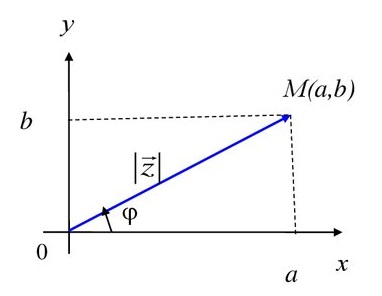
\includegraphics[width=0.34\textwidth]{images/complex.jpg}
\end{wrapfigure} Здесь $r$ -- длина радиус-вектора числа $z$ на плоскости комплексных чисел, $\varphi$ -- угол между радиус-вектором $z$ и действительной осью.
$$r = |z| = \sqrt{a^2 + b^2}$$
$$\cos{\varphi} = \frac{a}{r}, \;\;\;\; \sin{\varphi} = \frac{b}{r}$$

\addcontentsline{toc}{subsection}{ 2.4. Дайте определения модуля и аргумента комплексного числа. Что такое главное значение аргумента комплексного числа? }
\section*{\LARGE 2.4. Дайте определения модуля и аргумента комплексного числа. Что такое главное значение аргумента комплексного числа? }

Модулем комплексного числа $z$ называется $r = |z| = \sqrt{a^2 + b^2}$ -- величина, отражающая длину радиус-вектора точки $z$ в плоскости комплексных чисел.
\newline Аргументом комплексного числа называется угол между радиус-вектором точки $z$ и положительным направлением действительной оси. \underline{Главным} аргументом комплексного числа называется такой его аргумент который лежит в $(-\pi, \pi]$
$$ Arg(z) = arg(z) + 2\pi k,\;\;\; k \in \mathbb{Z},\; arg(z) \in (-\pi, \pi]$$

\addcontentsline{toc}{subsection}{ 2.5. Сложение, умножение комплексных чисел. Что происходит с аргументами и модулями комплексных чисел при умножении и при делении? }
\section*{\LARGE 2.5. Сложение, умножение комплексных чисел. Что происходит с аргументами и модулями комплексных чисел при умножении и при делении? }

Операции над комплексными числами выполняются по следующим правилам:
$$ (a_1, b_1) + (a_2, b_2) = (a_1 + a_2, b_1 + b_2) $$
$$ (a_1, b_1) \cdot (a_2, b_2) = (a_1a_2 - b_1b_2, a_1b_2 + a_2b_1) $$
В тригонометрической форме умножение и деление выглядят так:
$$ z_1 = r_1(\cos{\varphi_1} + i\sin{\varphi_1}) $$
$$ z_2 = r_2(\cos{\varphi_2} + i\sin{\varphi_2}) $$
$$ z_1 \cdot z_2 = r_1r_2(\cos{(\varphi_1 + \varphi_2)} + i\sin{(\varphi_1 + \varphi_2)}) $$
$$ \frac{z_1}{z_2} = \frac{r_1}{r_2}(\cos{(\varphi_1 - \varphi_2)} + i\sin{(\varphi_1 - \varphi_2)}) $$

\addcontentsline{toc}{subsection}{ 2.6. Что такое комплексное сопряжение? Как можно делить комплексные числа в алгебраической форме? }
\section*{\LARGE 2.6. Что такое комплексное сопряжение? Как можно делить комплексные числа в алгебраической форме? }

\begin{wrapfigure}{r}{0.2\textwidth}
    \centering
    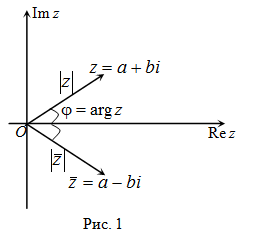
\includegraphics[width=0.2\textwidth]{images/sopr_complex.png}
\end{wrapfigure}
Сопряженным числом $\bar{z}$ для комплексного числа $z$ называется такое число, которое симметрично $z$ относительно вещественной оси.
$$z = a + ib, \;\; \bar{z} = a - ib$$. 
$$ $$ 
\newline Делить комплексные числа в алгебраической форме возможно путем домножение на сопряженное делителя:
$$
\frac{z_1}{z_2} = \frac{z_1 \bar{z_2}}{z_2 \bar{z_2}} = \frac{z_1 \bar{z_2}}{a_2^2 + b_2^2} = \frac{z_1 \bar{z_2}}{|z_2|^2}
$$

\addcontentsline{toc}{subsection}{ 2.7. Выпишите формулу Муавра.  }
\section*{\LARGE 2.7. Выпишите формулу Муавра.  }

Пусть $z = r(\cos{\varphi} + i\sin{\varphi})$, тогда
$$ z^n =  r^n(\cos{(n\varphi)} + i\sin{(n\varphi)}),\; n \in \mathbb{Z}$$

\addcontentsline{toc}{subsection}{ 2.8. Как найти комплексные корни $n$-ой степени из комплексного числа? Сделайте эскиз, на котором отметьте исходное число и все корни из него.  }
\section*{\LARGE 2.8. Как найти комплексные корни $n$-ой степени из комплексного числа? Сделайте эскиз, на котором отметьте исходное число и все корни из него.  }

Пусть $z = r(\cos{\varphi} + i\sin{\varphi})$, тогда корнем степени $n \in \mathbb{N}$ из $z$ называется множество
$$
\sqrt[n]{z} = \{\sqrt[n]{r}\left(\cos{\left(\frac{\varphi + 2\pi k}{n}\right) + i\sin{\left(\frac{\varphi + 2\pi k}{n}\right)}}\right),\; k = \overline{0, n-1}\}
$$
Пример: $\sqrt[6]{1}$
$$ 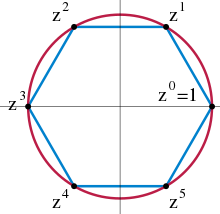
\includegraphics[width=0.35\textwidth]{images/squareroot.png}$$

\addcontentsline{toc}{subsection}{ 2.9. Сформулируйте основную теорему алгебры. Сформулируйте теорему Безу. }
\section*{\LARGE 2.9. Сформулируйте основную теорему алгебры. Сформулируйте теорему Безу. }

\underline{Основная теорема алгебры}:
$$
\forall f(z) = \sum_{i = 0}^n{a_iz^i} \ne const,\, a_i \in \mathbb{C} \;\; \exists z_0 \in C \::\: f(z_0) = 0
$$
\underline{Теорема Безу}:
\newline Остаток от деления $f(x)$ на $(x - a)$ равен $f(a)$.

\addcontentsline{toc}{subsection}{ 2.10. Выпишите формулу Эйлера. Выпишите выражения для синуса и косинуса через экспоненту.  }
\section*{\LARGE 2.10. Выпишите формулу Эйлера. Выпишите выражения для синуса и косинуса через экспоненту.  }

\underline{Формула Эйлера}:
$ e^{ix} = \cos{x} + i\sin{x} $
$$ \cos{x} = \frac{e^{ix} + e^{-ix}}{2}, \;\;\; \sin{x} = \frac{e^{ix} - e^{-ix}}{2i} $$

\addcontentsline{toc}{subsection}{ 2.11. Выпишите формулы Виета для многочлена третьей степени.  }
\section*{\LARGE 2.11. Выпишите формулы Виета для многочлена третьей степени.  }

Пусть $P(x) = ax^3 + bx^2 + cx + d$, $x_1, x_2, x_3$ -- корни многочлена $P(x)$.
$$ x_1 + x_2 + x_3 = -\frac{b}{a} $$
$$ x_1x_2 + x_2x_3 + x_1x_3 = \frac{c}{a} $$
$$ x_1x_2x_3 = -\frac{d}{a} $$

\addcontentsline{toc}{subsection}{ 2.12. Какие многочлены называются неприводимыми? }
\section*{\LARGE 2.12. Какие многочлены называются неприводимыми? }

Многочлен $P(x)$ называется \underline{приводимым}, если существуют многочлены 
\newline $g(x) \ne const$, $h(x) \ne const$ такие, что $P(x) = g(x) \cdot h(x)$ (это называется нетривиальное разложение) и \underline{неприводимым} в противном случае.

\addcontentsline{toc}{subsection}{ 2.13. Сформулируйте утверждение о разложении многочленов на неприводимые множители над полем комплексных чисел.  }
\section*{\LARGE 2.13. Сформулируйте утверждение о разложении многочленов на неприводимые множители над полем комплексных чисел.  }

Любой неконстантный многочлен степени $n$ над полем комплексных чисел можно разложить как 
$$ a(x - x_1)(x - x_2)...(x - x_n) $$
где $a \ne 0$, а значения $x_1, x_2, ...\,, x_n$ могут попарно совпадать.

\addcontentsline{toc}{subsection}{ 2.14. Дайте определение векторного произведения векторов в трехмерном пространстве. }
\section*{\LARGE 2.14. Дайте определение векторного произведения векторов в трехмерном пространстве. }

\begin{wrapfigure}{r}{0.2\textwidth}
    \centering
    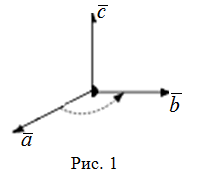
\includegraphics[width=0.2\textwidth]{images/right_troika.png}
\end{wrapfigure}
Вектор $\vec{c}$ назвается векторным произведением векторов $\vec{a}$ и $\vec{b}$ если:
\newline 1) $|\vec{c}| = |\vec{a}|\cdot|\vec{b}|\cdot\sin{\varphi}$, где $\varphi$ -- угол между $\vec{a}$ и $\vec{b}$
\newline 2) $\vec{c} \perp \vec{a},\, \vec{c} \perp \vec{b}$
\newline 3) $\vec{a}, \vec{b}, \vec{c}$ -- правая тройка векторов

\addcontentsline{toc}{subsection}{ 2.15. Выпишите формулу для вычисления векторного произведения в координатах, заданных в ортонормированном базисе.  }
\section*{\LARGE 2.15. Выпишите формулу для вычисления векторного произведения в координатах, заданных в ортонормированном базисе.  }

Пусть $\vec{i}, \vec{j}, \vec{k}$ задают правый ортонормированный базис, векторы $\vec{a}$ и $\vec{b}$ раскладываются в этом базисе следующим образом:
\newline $\vec{a} = a_i\vec{i} + a_j\vec{j} + a_k\vec{k}$
\newline $\vec{b} = b_i\vec{i} + b_j\vec{j} + b_k\vec{k}$
\newline Тогда 
$$\vec{a} \times \vec{b} = 
\begin{vmatrix}
\vec{i} & \vec{j} & \vec{k} \\
a_i & a_j & a_k \\
b_i & b_j & b_k
\end{vmatrix}$$

\addcontentsline{toc}{subsection}{ 2.16. Дайте определение смешанного произведения векторов. Как вычислить объем тетраэдра с помощью смешанного произведения?  }
\section*{\LARGE 2.16. Дайте определение смешанного произведения векторов. Как вычислить объем тетраэдра с помощью смешанного произведения?  }

Смешанным произведением векторов $\vec{a}, \vec{b}, \vec{c}$ называют число $<\vec{a}, \vec{b}, \vec{c}> = (\vec{a} \times \vec{b}, \vec{c})$ -- скалярное произведение $\vec{a} \times \vec{b}$ и $\vec{c}$.  Объем тетраэдра, построенного на векторах $\vec{a}, \vec{b}, \vec{c}$ равен
$$
V = \frac{1}{6}\,|<\vec{a}, \vec{b}, \vec{c}>|
$$

\addcontentsline{toc}{subsection}{ 2.17. Выпишите формулу для вычисления смешанного произведения в координатах, заданных в ортонормированном базисе.  }
\section*{\LARGE 2.17. Выпишите формулу для вычисления смешанного произведения в координатах, заданных в ортонормированном базисе.  }

Пусть $\vec{i}, \vec{j}, \vec{k}$ задают правый ортонормированный базис, векторы $\vec{a}$, $\vec{b}$ и $\vec{c}$ раскладываются в этом базисе следующим образом:
\newline $\vec{a} = a_i\vec{i} + a_j\vec{j} + a_k\vec{k}$
\newline $\vec{b} = b_i\vec{i} + b_j\vec{j} + b_k\vec{k}$
\newline $\vec{c} = c_i\vec{i} + c_j\vec{j} + c_k\vec{k}$
\newline Тогда 
$$<\vec{a}, \vec{b}, \vec{c}> = 
\begin{vmatrix}
a_i & a_j & a_k \\
b_i & b_j & b_k \\
c_i & c_j & c_k \\
\end{vmatrix}$$

\addcontentsline{toc}{subsection}{ 2.18. Сформулируйте критерий компланарности трех векторов с помощью смешанного произведения. }
\section*{\LARGE 2.18. Сформулируйте критерий компланарности трех векторов с помощью смешанного произведения. }

Векторы $\vec{a}$, $\vec{b}$ и $\vec{c}$ компланарны тогда и только тогда, когда $<\vec{a}, \vec{b}, \vec{c}> = 0$.

\addcontentsline{toc}{subsection}{ 2.19. Что такое уравнение поверхности и его геометрический образ? }
\section*{\LARGE 2.19. Что такое уравнение поверхности и его геометрический образ? }

Уравнение $F(x, y, z) = 0$ называют уравнением поверхности $S$, если этому уравнению удовлетворяют координаты каждой из точек, лежащих на $S$, и не удовлетворяют никакие точки, не лежащие на $S$. При этом $S$ называется геометрическим образом уравнения $F(x, y, z) = 0$.

\addcontentsline{toc}{subsection}{ 2.20. Сформулируйте теорему о том, что задает любое линейное уравнение на координаты точки в трехмерном пространстве.}
\section*{\LARGE 2.20. Сформулируйте теорему о том, что задает любое линейное уравнение на координаты точки в трехмерном пространстве.  }

Любое уравнение вида $Ax + By + Cz + D = 0$, где $A^2 + B^2 + C^2 > 0$ (т.е. линейное уравнение), определяет плоскость в пространстве $\mathbb{R}^3$.

\addcontentsline{toc}{subsection}{ 2.21. Что такое нормаль к плоскости?  }
\section*{\LARGE 2.21. Что такое нормаль к плоскости?  }

Нормалью к плоскости $\alpha$ называется такой вектор $\vec{n}$, что $\vec{n} \perp \alpha$. В частности, если $\alpha : Ax + By + Cz + D = 0$, то $\vec{n} = (A, B, C)$ является вектором нормали к $\alpha$.

\addcontentsline{toc}{subsection}{ 2.22. Выпишите формулу для расстояния от точки до плоскости. }
\section*{\LARGE 2.22. Выпишите формулу для расстояния от точки до плоскости. }

Пусть $P(x_0, y_0, z_0)$ -- точка, $Ax + By + Cz + D = 0$ -- уравнение плоскости $\alpha$. Тогда 
$$
\rho(P, \alpha) = \frac{|Ax_0 + By_0 + Cz_0 + D|}{\sqrt{A^2 + B^2 + C^2}} 
$$

\addcontentsline{toc}{subsection}{ 2.23. Общие уравнения прямой. Векторное уравнение прямой. Параметрические и канонические уравнения прямой.  }
\section*{\LARGE 2.23. Общие уравнения прямой. Векторное уравнение прямой. Параметрические и канонические уравнения прямой.  }

Общие уравнения прямой задают прямую как пересечение двух плоскостей:
$$
\begin{cases}
A_1x + B_1y + C_1z + D_1 = 0 \\
A_2x + B_2y + C_2z + D_2 = 0
\end{cases}
$$
Векторное уравнение прямой: $\vec{r}(t) = \vec{r_0} + \vec{s}t$
\newline где $\vec{r}(t)$ -- радиус-вектор \underline{любой} точки прямой
\newline $\vec{r_0}$ -- радиус-вектор \underline{определённой} точки прямой
\newline $\vec{s}$ -- направляющий вектор прямой.
\newline $ $
\newline Параметрические уравнения прямой:
$$
\begin{cases}
x = x_0 + s_x\cdot t \\
y = y_0 + s_y\cdot t \\
z = z_0 + s_z\cdot t \\
\end{cases}
$$
где $M(x_0, y_0, z_0)$ -- точка прямой, $\vec{s}(s_x, s_y, s_z)$ -- направляющий вектор прямой.
\newline Каноническое уравнение прямой (\textit{преобразованное параметрическое}):
$$
\frac{x - x_0}{s_x} = \frac{y - y_0}{s_y} = \frac{z - z_0}{s_z}
$$

\addcontentsline{toc}{subsection}{ 2.24. Выпишите формулу для вычисления расстояния между двумя скрещивающимися прямыми.  }
\section*{\LARGE 2.24. Выпишите формулу для вычисления расстояния между двумя скрещивающимися прямыми.  }

Пусть $L_1, L_2$ -- скрещивающиеся прямые, $\vec{s_1}, \vec{s_2}$ -- их направляющие векторы, $M_1 \in L_1, M_2 \in L_2$ -- произвольные точки на прямых. Тогда 
$$
\rho(L_1, L_2) = \frac{<\vec{s_1}, \vec{s_2}, \overrightarrow{M_1M_2}>}{|\vec{s_1} \times \vec{s_2}|} \;\; (\;= \frac{V}{S_{\mbox{осн}}})
$$

\addcontentsline{toc}{subsection}{ 2.25. Какие бинарные операции называются ассоциативными, а какие коммутативными?  }
\section*{\LARGE 2.25. Какие бинарные операции называются ассоциативными, а какие коммутативными?  }

Операция $\times$ называется:
\newline - ассоциативной, если $\forall x,y,z \;\; (x \times y) \times z = x \times (y \times z)$
\newline - коммутативной, если $\forall x,y \;\; x \times y = y \times x$

\addcontentsline{toc}{subsection}{ 2.26. Дайте определения полугруппы и моноида. Приведите примеры. }
\section*{\LARGE 2.26. Дайте определения полугруппы и моноида. Приведите примеры. }

\underline{Полугруппа} -- группоид (\textit{множество с заданной на нём операцией}), операция которой ассоциативна. Пример: $(\mathbb{N}, +)$.
\newline \underline{Моноид} -- полугруппа, в которой есть нейтральный элемент.
\newline Примеры: $(\mathbb{N}\cup \{0\}, +),\, (\mathbb{N}, \cdot)$.

\addcontentsline{toc}{subsection}{ 2.27. Сформулируйте определение группы. Приведите пример. }
\section*{\LARGE 2.27. Сформулируйте определение группы. Приведите пример. }

Группа -- множество с заданной на нём ассоциативной операцией, имеющая нейтральный элемент, причём все элементы являются обратимыми, т.е. 
$$
\forall g \in G \; \exists a^{-1} \in G : a \cdot a^{-1} = a^{-1} \cdot a = e \; \mbox{(нейтральный элемент)}
$$
Иначе говоря -- моноид, все элементы которого обратимы.
\newline Пример: $GL_n$ -- множество всех невырожденных матриц $n \times n$ с операцией умножения.

\addcontentsline{toc}{subsection}{ 2.28. Что такое симметрическая группа? Укажите число элементов в ней.  }
\section*{\LARGE 2.28. Что такое симметрическая группа? Укажите число элементов в ней.  }

Симметрическая группа -- множество всех подстановок длины $n$ с операцией композиции. Обозначается $S_n$, число элементов $n!$.

\addcontentsline{toc}{subsection}{ 2.29. Что такое общая линейная и специальная линейная группы?  }
\section*{\LARGE 2.29. Что такое общая линейная и специальная линейная группы?  }

Общая линейная группа ($GL_n$) -- множество всех невырожденных матриц $n \times n$ с операцией умножения. Запись $GL_n(\mathbb{F})$ означает, что элементы матрицы принадлежат полю (кольцу) $\mathbb{F}$, например $GL_n(\mathbb{R})$.
\newline Специальная линейная группа -- множество всех матриц $n \times n$ с определителем, равным 1, и операцией умножения:
$$
SL_n(\mathbb{F}) = \{A \in GL_n(\mathbb{F}) \:|\: \det{A} = 1\}
$$

\addcontentsline{toc}{subsection}{ 2.30. Сформулируйте определение абелевой группы. Приведите пример. }
\section*{\LARGE 2.30. Сформулируйте определение абелевой группы. Приведите пример. }

Абелева группа -- группа, операция которой коммутативна. Пример:$(\mathbb{Z}, +)$.

\addcontentsline{toc}{subsection}{ 2.31. Дайте определение подгруппы. Приведите пример группы и её подгруппы.  }
\section*{\LARGE 2.31. Дайте определение подгруппы. Приведите пример группы и её подгруппы.  }

Подмножество $H$ множества группы $G$ с определённой на нём операцией $G$ называется подгруппой, если она сама является группой относительно данной операции. 
\newline Подмножество $H$ является подгруппой $G$ тогда и только тогда, когда выполняются все три условия:
\newline 1) $H$ содержит нейтральный элемент $G$;
\newline 2) $\forall h_1, h_2 \in H \;\; h_1 \cdot h_2 \in H$;
\newline 3) $\forall h \in H \: \exists h^{-1} \in H : h \cdot h^{-1} = h^{-1} \cdot h = e$;
\newline Пример: $SL_n(\mathbb{R})$ -- подгруппа $GL_n(\mathbb{R})$.

\addcontentsline{toc}{subsection}{ 2.32. Дайте определение гомоморфизма групп. Приведите пример.  }
\section*{\LARGE 2.32. Дайте определение гомоморфизма групп. Приведите пример.  }

Отображение $f : G_1 \rightarrow G_2$ группы $(G_1, \circ)$ в группу $(G_2, \diamond)$ называется гомоморфизмом, если $\forall a, b \in G_1 \; f(a \circ b) = f(a) \diamond f(b)$. 
\newline Пример: $\ln : (\mathbb{R}^+ \backslash \{0\}, \cdot) \rightarrow (\mathbb{R}, +)$ -- гомоморфизм, так как $\ln{(ab)} = \ln{a} + \ln{b}$.

\addcontentsline{toc}{subsection}{ 2.33. Что такое ядро гомоморфизма групп? Приведите пример.  }
\section*{\LARGE 2.33. Что такое ядро гомоморфизма групп? Приведите пример.  }

Ядром гомоморфизма $f : G_1 \rightarrow G_2$ называется множество всех элементов первой группы, которые переходят в нейтральный элемент второй: $$Kerf = \{g \in G_1 \:|\: f(g) = e_2\}$$
Пример: для гомоморфизма $\det : GL_n(\mathbb{R}) \rightarrow \mathbb{R}^*$ 
\newline $Ker(\det) = SL_n(\mathbb{R}) = \{A \in GL_n(\mathbb{R}) \:|\: \det{A} = 1\}$.

\addcontentsline{toc}{subsection}{ 2.34. Дайте определение изоморфизма групп. Приведите пример. }
\section*{\LARGE 2.34. Дайте определение изоморфизма групп. Приведите пример. }

Изоморфизм -- биективный гомоморфизм. 
\newline Пример: $f : (\mathbb{R}, +) \rightarrow (\mathbb{R}^+, \cdot), \, f(x) = e^x$.

\addcontentsline{toc}{subsection}{ 2.35. Сформулируйте определение циклической группы. Приведите пример.  }
\section*{\LARGE 2.35. Сформулируйте определение циклической группы. Приведите пример.  }

$(G, \circ)$ -- циклическая группа, если $\exists g_1 \in G \; \forall g \in G \; g = g_1 \circ ... \circ g_1$ (все элементы порождены каким-то элементом). Обозначение: $\left<g\right>$. Пример: $(\mathbb{Z}_n, +)$, где $\mathbb{Z}_n = \{0, 1, ... \,, n - 1\}$ -- циклическая группа ($g_1 = 1$).

\addcontentsline{toc}{subsection}{ 2.36. Дайте определение порядка элемента.  }
\section*{\LARGE 2.36. Дайте определение порядка элемента.  }

Порядок элемента $g \in (G, \circ)$ -- наименьшее $p \in \mathbb{N} \:|\: g^p = e$, где $g^p = \underbrace{g \circ ... \circ g}_{p}$. Обозначение: $ord(g)$.

\addcontentsline{toc}{subsection}{ 2.37. Сформулируйте утверждение о связи порядка элемента, порождающего циклическую группу, с порядком группы.  }
\section*{\LARGE 2.37. Сформулируйте утверждение о связи порядка элемента, порождающего циклическую группу, с порядком группы.  }

Пусть $\left<g\right>$ -- группа, порожденная элементом $g$, тогда $ord(g) = |\left<g\right>|$.

\addcontentsline{toc}{subsection}{ 2.38. Сколько существует, с точностью до изоморфизма, циклических групп данного порядка? }
\section*{\LARGE 2.38. Сколько существует, с точностью до изоморфизма, циклических групп данного порядка? }

Для каждого натурального порядка $n$ существует ровно одна циклическая группа, с точностью до изоморфизма.

\addcontentsline{toc}{subsection}{ 2.39. Что такое группа диэдра? Что такое знакопеременная группа? Укажите число элементов в них. }
\section*{\LARGE 2.39. Что такое группа диэдра? Что такое знакопеременная группа? Укажите число элементов в них. }

Группа диэрдра -- группа симметрий правильного $n$-угольника. Обозначение: $D_n$, $|D_n| = 2n$.
$$ D_n = \{r, s \:|\: r^n = 1,\, s^2 = 1,\, s^{-1}rs = r^{-1}\} \; (r - rotation, s - symmetry)$$
\newline Знакопеременная группа -- все чётные подстановки длины $n$. Обозначение: $A_n$. $A_n \subset S_n$, $|A_n| = \frac{n!}{2}$.

\addcontentsline{toc}{subsection}{ 2.40. Сформулируйте утверждение о том, какими могут быть подгруппы группы целых чисел по сложению.  }
\section*{\LARGE 2.40. Сформулируйте утверждение о том, какими могут быть подгруппы группы целых чисел по сложению.  }

Любая подгруппа группы целых чисел по сложению имеет вид $G = kZ$, где $k \in \mathbb{N}\cup\{0\}$. Т.е. это группа всех чисел, кратных определенному значению.

\addcontentsline{toc}{subsection}{ 2.41. Дайте определение левого смежного класса по некоторой подгруппе. }
\section*{\LARGE 2.41. Дайте определение левого смежного класса по некоторой подгруппе. }

Пусть $G$ -- группа, $H \subseteq G$, $g \in G$. Левым смежным классом элемента $g$ по подгруппе $H$ называется множество $gH = \{gh \:|\: h \in H\}$.

\addcontentsline{toc}{subsection}{ 2.42. Что такое индекс подгруппы? }
\section*{\LARGE 2.42. Что такое индекс подгруппы? }

Индексом подгруппы $H \subseteq G$ называется число различных левых смежных классов группы $G$ по подгруппе $H$. Обозначение: $[G : H]$.

\addcontentsline{toc}{subsection}{ 2.43. Сформулируйте теорему Лагранжа. }
\section*{\LARGE 2.43. Сформулируйте теорему Лагранжа. }

Пусть $G$ -- конечная группа, $H \subseteq G$. Тогда $|G| = |H|[G : H]$, где $[G : H]$ -- индекс подгруппы, т.е. число левых смежных классов по $H$.

\addcontentsline{toc}{subsection}{ 2.44. Сформулируйте две леммы, которые нужны для доказательства теоремы Лагранжа. }
\section*{\LARGE 2.44. Сформулируйте две леммы, которые нужны для доказательства теоремы Лагранжа. }

\underline{Лемма 1}:
\newline $\forall g_1, g_2 \in G \; (g_1H = g_2H) \oplus (g_1H \cap g_1H = \varnothing)$
\newline \underline{Лемма 2}:
\newline $\forall g \in G \: \forall H \subseteq G \;\; |gH| = |H|$

\newpage
\addcontentsline{toc}{section}{\Large \underline{Модуль 3} }
\section*{\LARGE\centering \underline{Модуль 3}}

\addcontentsline{toc}{subsection}{ 3.1. Сформулируйте критерий нормальности подгруппы, использующий сопряжение.  }
\section*{\LARGE 3.1. Сформулируйте критерий нормальности подгруппы, использующий сопряжение.}
Пусть $H \subseteq G$ -- подгруппа в группе $G$. Тогда если $gHg^{-1} = \{ghg^{-1}\;|\;h\in H\}\;\;\;$ 3 условия эквивалентны:
\newline \indent 1. $H$ нормальна
\newline \indent 2. $\forall g \in G \; gHg^{-1} \subseteq H $
\newline \indent 3. $\forall g \in G \; gHg^{-1} = H $

\addcontentsline{toc}{subsection}{ 3.2. Дайте определение факторгруппы  }
\section*{\LARGE 3.2. Дайте определение факторгруппы.}
Факторгруппа -- множество смежных классов $G$ по нормальной подгруппе $H\triangleleft G$ с определённой на ней операцией умножения: $(g_1H)\cdot(g_2H) = g_1g_2H$. \newline Обозначение: $G/H$ -- факторгруппа $G$ по нормальной подгруппе $H$.

\addcontentsline{toc}{subsection}{ 3.3. Что такое естественный гомоморфизм?  }
\section*{\LARGE 3.3. Что такое естественный гомоморфизм?}
Естественный гомоморфизм для группы $G$ -- отображение $f : G \rightarrow G/H$ такое, что $f(g) = gH \; \forall g \in G$.

\addcontentsline{toc}{subsection}{ 3.4. Сформулируйте критерий нормальности подгруппы, использующий понятие ядра гомоморфизма.  }
\section*{\LARGE 3.4. Сформулируйте критерий нормальности подгруппы, использующий понятие ядра гомоморфизма.}
$H\triangleleft G \Leftrightarrow \exists f : G \rightarrow G'$ -- гомоморфизм, причём $Kerf = H$.

\addcontentsline{toc}{subsection}{ 3.5. Сформулируйте теорему о гомоморфизме групп. Приведите пример.  }
\section*{\LARGE 3.5. Сформулируйте теорему о гомоморфизме групп. Приведите пример.}
Пусть $f : G_1 \rightarrow G_2$ -- гомоморфизм групп,
\newline $Imf = \{g_2 \in G_2 \:|\: \exists g_1 \in G_1 : f(g_1) = g_2\}$ (образ группы $G$ по $f$), 
\newline $Kerf = \{g_1 \in G_1 \:|\: f(g_1) = e_2\}$ (ядро гомоморфизма $f$).
\newline Тогда $G_1/Kerf \cong Imf$.
\newline \underline{Пример:}
\newline Пусть $f : \mathbb{Z} \rightarrow \mathbb{Z}_n$ такое, что $\forall z \in \mathbb{Z} \; f(z) = z \:\%\: n$ (остаток от деления на $n$). Очевидно, $Kerf = n\mathbb{Z}$ -- числа, кратные $n$. Тогда $\mathbb{Z}/n\mathbb{Z} = \mathbb{Z}_n$.

\addcontentsline{toc}{subsection}{ 3.6. Что такое прямое произведение групп?  }
\section*{\LARGE 3.6. Что такое прямое произведение групп?}
Прямое произведение групп -- группа из всех пар элементов групп с операцией поэлементого умножения.
$$(G, +) \times (H, \circ) = \{(g, h) \:|\: g \in G,\, h \in H\},\;\; (g_1, h_1)\times(g_2, h_2) = (g_1 + g_2, h_1 \circ h_2)$$

\addcontentsline{toc}{subsection}{ 3.7. Сформулируйте определение автоморфизма и внутреннего автоморфизма.  }
\section*{\LARGE 3.7. Сформулируйте определение автоморфизма и внутреннего автоморфизма. }
Автоморфизм -- изоморфное отображение группы в себя. Внутренний автоморфизм -- отображение $I_a : g \mapsto aga^{-1}$, где $a,g \in G$ ($a$ фиксированный).

\addcontentsline{toc}{subsection}{ 3.8. Что такое центр группы? Приведите пример.  }
\section*{\LARGE 3.8. Что такое центр группы? Приведите пример. }
Центр группы $G$ -- подгруппа коммутирующих элементов, т.е. 
\newline $Z(G) = \{a \in G \:|\: \forall b \in G \; ab = ba\}$.
\newline Для абелевых групп центр группы совпадает с самой группой. Например, 
\newline классы вычетов: $\mathbb{Z}(\mathbb{Z}_n) = \mathbb{Z}_n$.

\addcontentsline{toc}{subsection}{ 3.9. Чему изоморфна факторгруппа группы по её центру?  }
\section*{\LARGE 3.9. Чему изоморфна факторгруппа группы по её центру? }
$$G/Z(G) \cong Inn(G)$$
$Inn$ -- подгруппа всех внутренних автоморфизмов: $Inn = \{g \mapsto aga^{-1}\,|\, a,g \in G\}$.

\addcontentsline{toc}{subsection}{ 3.10. Сформулируйте теорему Кэли.  }
\section*{\LARGE 3.10. Сформулируйте теорему Кэли. }
Любая конечная группа порядка $n$ изоморфна некоторой подгруппе группы перестановок $S_n$.

\addcontentsline{toc}{subsection}{ 3.11. Дайте определение кольца.  }
\section*{\LARGE 3.11. Дайте определение кольца. }
Кольцо -- множество $K \ne \varnothing$, на котором заданы 2 бинарные операции $+$ и $\cdot$ такие, что
\newline\indent 1. $(K, +)$ -- абелева группа;
\newline\indent 2. $(K, \cdot)$ -- полугруппа;
\newline\indent 3. Умножение дистрибутивно относительно сложения: $\forall a,b,c \in K$
$$
\begin{cases}
a(b + c) = ab + ac \\
(a + b)c = ac + bc 
\end{cases}
$$
Обозначение: $(K, +, \cdot)$.
\newline \underline{\textit{Для профилактики:}}
\newline Группоид -- замкнутость относительно операции.
\newline Полугруппа -- ассоциативность.
\newline Моноид -- нейтральный элемент.
\newline Группа -- обратные элементы.

\addcontentsline{toc}{subsection}{ 3.12. Что такое коммутативное кольцо? Приведите примеры коммутативного и некоммутативного колец.  }
\section*{\LARGE 3.12. Что такое коммутативное кольцо? Приведите примеры коммутативного и некоммутативного колец. }
Коммутативное кольцо -- кольцо с коммутативным умножением: $\forall a,b \in K \newline ab = ba$
\newline \underline{Примеры:}
\newline Коммутативное -- $(\mathbb{Z}, +, \cdot)$.
\newline Некоммутативное -- $(M_n(\mathbb{R}), +, \times)$ -- полное матричное кольцо $n\times n$ над $\mathbb{R}$.

\addcontentsline{toc}{subsection}{ 3.13. Дайте определение делителей нуля.  }
\section*{\LARGE 3.13. Дайте определение делителей нуля. }
Если $\exists a,b \in K \::\: (a \ne 0 \ne b) \wedge (a\cdot b = 0)$, то $a$ -- левый делитель нуля, $b$ -- правый делитель нуля. 

\addcontentsline{toc}{subsection}{ 3.14. Дайте определение целостного кольца. Приведите пример.  }
\section*{\LARGE 3.14. Дайте определение целостного кольца. Приведите пример. }
Целостное кольцо -- коммутативное кольцо без делителей нуля и с единицей (не равной нулю). Целостное кольцо $\equiv$ область целостности.

\addcontentsline{toc}{subsection}{ 3.15. Сформулируйте критерий целостности для нетривиального коммутативного кольца с единицей.  }
\section*{\LARGE 3.15. Сформулируйте критерий целостности для нетривиального коммутативного кольца с единицей. }
Нетривиальное коммутативное кольцо $K$ является целостным тогда и только тогда, когда в нем выполняется закон сокращения, т.е. $\forall a,b,c \in K$
$$
\begin{cases}
(ab = ac)\wedge(a \ne 0) \Rightarrow b = c \\
(ac = bc)\wedge(c\ne 0) \Rightarrow a = b
\end{cases}
$$

\addcontentsline{toc}{subsection}{ 3.16. Какие элементы кольца называются обратимыми?  }
\section*{\LARGE 3.16. Какие элементы кольца называются обратимыми? }
Элемент $a$ кольца $K$ называется обратимым, если $\exists a^{-1} \in K : a\cdot a^{-1} = a^{-1}\cdot a = 1$.

\addcontentsline{toc}{subsection}{ 3.17. Дайте определение поля. Приведите три примера.  }
\section*{\LARGE 3.17. Дайте определение поля. Приведите три примера. }
Поле -- коммутативное кольцо с единицей (не равной нулю), в котором каждый элемент $a \ne 0$ обратим.
\newline \underline{Примеры:} $\mathbb{R}, \, \mathbb{C}, \, \mathbb{Q}$ с операциями $(+, \cdot)$.

\addcontentsline{toc}{subsection}{ 3.18. Дайте определение подполя. Приведите пример пары: поле и его подполе.  }
\section*{\LARGE 3.18. Дайте определение подполя. Приведите пример пары: поле и его подполе. }
Подполе -- подмножество поля, которое само является полем относительно операций поля.
\newline \underline{Пример:} $\mathbb{Q} \subset \mathbb{R}$ -- поле рациональных чисел является подполем поля действительных чисел.   

\addcontentsline{toc}{subsection}{ 3.19. Дайте определение характеристики поля. Привести примеры: поля конечной положительной характеристики и поля нулевой характеристики.  }
\section*{\LARGE 3.19. Дайте определение характеристики поля. Привести примеры: поля конечной положительной характеристики и поля нулевой характеристики. }
Характеристикой поле $P$ (обозначение: char$P$) называется наименьшее $p \in \mathbb{N}$ такое, что $\underbrace{1 + 1 + ... + 1}_{p} = 0$. Если такого $p$ не существует, то char$P$ = 0.
\newline \underline{Примеры: }
\newline -- Если $p$ -- простое, то char$\mathbb{Z}_p = p$;
\newline -- char$\mathbb{R} = 0$;

\addcontentsline{toc}{subsection}{ 3.20. Сформулируйте утверждение о том, каким будет простое подполе в зависимости от характеристики.  }
\section*{\LARGE 3.20. Сформулируйте утверждение о том, каким будет простое подполе в зависимости от характеристики. }
Пусть $P$ -- поле, $P_0$ -- его простое подполе. Тогда 
\newline\indent 1) char$P = p > 0 \Rightarrow P_0 \cong \mathbb{Z}_p$;
\newline\indent 2) char$P = 0 \Rightarrow P_0 \cong \mathbb{Q}$;

\addcontentsline{toc}{subsection}{ 3.21. Дайте определение идеала. Что такое главный идеал?  }
\section*{\LARGE 3.21. Дайте определение идеала. Что такое главный идеал? }
Подмножество $I$ кольца $K$ называется идеалом, если 
\newline\indent 1. $(I, +) \subseteq (K, +)$.
\newline\indent 2. $\forall a \in I\,\forall k \in K \;\; ak \in I \wedge ka \in I$.
\newline Идеал называется главным, если $\exists a \in K : I = aK = \left<a\right>$.

\addcontentsline{toc}{subsection}{ 3.22. Сформулируйте определение гомоморфизма колец.  }
\section*{\LARGE 3.22. Сформулируйте определение гомоморфизма колец. }
Отображение $f : (K_1, +, \cdot) \rightarrow (K_2, \oplus, \odot)$ называется гомоморфизмом колец $K_1, K_2$, если 
\newline\indent 1. $\forall a,b \in K_1 \;\; f(a + b) = f(a) \oplus f(b)$
\newline\indent 2. $\forall a,b \in K_1 \;\; f(a \cdot b) = f(a) \odot f(b)$

\addcontentsline{toc}{subsection}{ 3.23. Сформулируйте теорему о гомоморфизме колец. Приведите пример.  }
\section*{\LARGE 3.23. Сформулируйте теорему о гомоморфизме колец. Приведите пример. }
Пусть $f : K_1 \rightarrow K_2$ -- гомоморфизм колец, $Imf$ -- гомоморфный образ $K_2$ по $f$. Тогда
$$K_1 / Kerf \cong Imf$$
\underline{Пример:}
\newline Пусть $f : \mathbb{Z} \rightarrow \mathbb{Z}_n$ такое, что $\forall z \in \mathbb{Z} \; f(z) = z \:\%\: n$ (остаток от деления на $n$). Очевидно, $Kerf = n\mathbb{Z}$ -- числа, кратные $n$. Тогда $\mathbb{Z}/n\mathbb{Z} = \mathbb{Z}_n$.

\addcontentsline{toc}{subsection}{ 3.24. Сформулируйте критерий того, что кольцо вычетов по модулю $n$ является полем.  }
\section*{\LARGE 3.24. Сформулируйте критерий того, что кольцо вычетов по модулю $n$ является полем. }
Кольцо вычетов $\mathbb{Z}_n$ является полем $\Leftrightarrow n$ -- простое. 

\addcontentsline{toc}{subsection}{ 3.25. Сформулируйте теорему о том, когда факторкольцо кольца многочленов над полем само является полем.  }
\section*{\LARGE 3.25. Сформулируйте теорему о том, когда факторкольцо кольца многочленов над полем само является полем. }
Факторкольцо $P[x] / \langle f(x)\rangle$ является полем $\Leftrightarrow f(x)$ неприводимо над полем $P$.

\addcontentsline{toc}{subsection}{ 3.26. Дайте определение алгебраического элемента над полем.  }
\section*{\LARGE 3.26. Дайте определение алгебраического элемента над полем. }
Элемент поля $\alpha \in P_2$ называется алгебраическим над полем $P_1 \subseteq P_2$, если $\exists f(x) \in P_1[x] : (f(x) \ne 0) \wedge (f(\alpha) = 0)$.

\addcontentsline{toc}{subsection}{ 3.27. Сформулируйте утверждение о том, что любое конечное поле может быть реализовано как факторкольцо кольца многочленов по некоторому идеалу.  }
\section*{\LARGE 3.27. Сформулируйте утверждение о том, что любое конечное поле может быть реализовано как факторкольцо кольца многочленов по некоторому идеалу. }
Любое конечное поле $\mathbb{F}_q$ (где $q = p^n,\, p$ -- простое) можно реализовать в виде $\mathbb{Z}_p[x] / \langle h(x) \rangle$, где $h(x)$ -- неприводимый многочлен степени $n$ над $\mathbb{Z}_p$.

\addcontentsline{toc}{subsection}{ 3.28. Сформулируйте утверждение о том, сколько элементов может быть в конечном поле.  }
\section*{\LARGE 3.28. Сформулируйте утверждение о том, сколько элементов может быть в конечном поле. }
Число элементов в конечном поле всегда $p^n$, где $p$ -- простое, $n \in \mathbb{N}$.

\addcontentsline{toc}{subsection}{ 3.29. Дайте определение линейного (векторного) пространства.  }
\section*{\LARGE 3.29. Дайте определение линейного (векторного) пространства. }
Пусть $F$ -- поле, $V$ -- произвольное множество, на котором корректно заданы 2 операции: сложение и умножение на скаляр (элемент поля $\mathbb{F}$). Иными словами, $\forall x, y \in V \;\; \forall \alpha \in \mathbb{F}$
$$
\begin{cases}
\exists z = x + y, \; z \in V \\
\exists w = \alpha x, \; w \in V
\end{cases}
$$
Множество $V$ называют линейным (векторным) пространством, если выполнены следующие 8 условий:
\newline\indent 1. $\forall x,y,z \in V \;\; x + (y + z) = (x + y) + z$ -- ассоциативность сложения;
\newline\indent 2. $\exists 0 \in V\: \forall x \in V : x + 0 = 0 + x = x$ -- нейтральный эл-т по сложению;
\newline\indent 3. $\forall x \in V \: \exists (-x) \in V : x + (-x) = (-x) + x = 0$ -- обратный эл-т по сложению;
\newline\indent 4. $\forall x, y \in V \;\; x + y = y + x$ -- коммутативность сложения;
\newline \underline{1-4 свойства -- абелева группа по сложению}
\newline\indent 5. $\exists 1 \in \mathbb{F} : \forall x \in V \;\; x \cdot 1 = 1 \cdot x = x$ -- нейтральный эл-т по умножению;
\newline\indent 6. $\forall x \in V \: \forall \alpha, \beta \in \mathbb{F} \;\; (\alpha\beta)x = \alpha(\beta x)$ -- ассоциативность умножения на число;
\newline\indent 7. $\forall x, y \in V \: \forall \alpha, \beta \in \mathbb{F} \;\;(\alpha + \beta)x = \alpha x + \beta x$ -- дистрибутивность 1;
\newline\indent 8. $\forall x, y \in V \: \forall \alpha, \beta \in \mathbb{F} \;\;\alpha(x + y) = \alpha x + \alpha y$ -- дистрибутивность 2;

\addcontentsline{toc}{subsection}{ 3.30. Дайте определение базиса линейного (векторного) пространства.  }
\section*{\LARGE 3.30. Дайте определение базиса линейного (векторного) пространства. }
Базисом линейного пространства $V$ называется упорядоченный набор векторов $b_1, ..., b_n \in V$ такой, что:
\newline \indent 1) $b_1, ..., b_n$ -- линейно независимы;
\newline \indent 2) любой вектор из $V$ представим в виде линейной комбинации $b_1, ..., b_n$:
\newline\indent $\forall x \in V \;\; x = \lambda_1b_1 + ... + \lambda_nb_n,\: \lambda_i \in \mathbb{F}$, причём \underline{единственным} образом;

\addcontentsline{toc}{subsection}{ 3.31. Что такое размерность пространства?  }
\section*{\LARGE 3.31. Что такое размерность пространства? }
Размерность пространства $V$ -- максимальное количество линейно независимых векторов в нём. Обозначение: dim$V$.

\addcontentsline{toc}{subsection}{ 3.32. Дайте определение матрицы перехода от старого базиса линейного пространства к новому.  }
\section*{\LARGE 3.32. Дайте определение матрицы перехода от старого базиса линейного пространства к новому. }
Пусть в линейном пространстве есть 2 базиса $A = \{a_1, ..., a_n\}$ и $B = \{b_1, ..., b_n\}$. Разложим векторы $B$ по базису $A$:
$$
\begin{cases}
b_1 = t_{11}a_1 + ... + t_{n1}a_n \\
... \\
b_n = t_{1n}a_1 + ... + t_{nn}a_n
\end{cases}
$$
где $t_{ij} \in \mathbb{F}$. Тогда матрицей перехода от базиса $A$ к базису $B$ называется матрица 
$$
T_{a \rightarrow b} = 
\begin{pmatrix}
t_{11} & ... & t_{1n} \\
... & ... & ... \\
t_{n1} & ... & t_{nn}
\end{pmatrix}
$$
Используется так: $x^b = T_{A \rightarrow B}^{-1} x^a$.

\addcontentsline{toc}{subsection}{ 3.33. Выпишите формулу для описания изменения координат вектора при изменении базиса.  }
\section*{\LARGE 3.33. Выпишите формулу для описания изменения координат вектора при изменении базиса. }
Пусть $x \in V,\, A$ и $B$ -- базисы в $V, \, x^a = (x_1^a, ..., x_n^a)^T, \, x^b = (x_1^b, ..., x_n^b)^T$ -- столбцы координат вектора $x$ в базисах $A$ и $B$ соответственно. Тогда $x^b = T_{A \rightarrow B}^{-1} x^a$.

\addcontentsline{toc}{subsection}{ 3.34. Дайте определение подпространства в линейном пространстве.  }
\section*{\LARGE 3.34. Дайте определение подпространства в линейном пространстве. }
Подмножество $L$ линейного пространства $V$ называется подпространством, если оно само является пространством относительно операций в $V$.

\addcontentsline{toc}{subsection}{ 3.35. Дайте определения линейной оболочки конечного набора векторов и ранга системы векторов.  }
\section*{\LARGE 3.35. Дайте определения линейной оболочки конечного набора векторов и ранга системы векторов. }
Линейной оболочной системы векторов $a_1, ..., a_k$ называется множество $L(a_1, ..., a_k) = \; = \{\lambda_1a_1 + ... + \lambda_ka_k \;|\; \lambda_i \in \mathbb{F} \}$ -- множество всех линейных комбинаций векторов $a_1, ..., a_k$.
\newline Рангом системы векторов $a_1, ..., a_k$ в линейном пространстве называется размерность линейной оболочки системы: $Rg(a_1, ..., a_k) = \mbox{dim}L(a_1,...,a_k)$.

\addcontentsline{toc}{subsection}{ 3.36. Дайте определения суммы и прямой суммы подпространств.  }
\section*{\LARGE 3.36. Дайте определения суммы и прямой суммы подпространств. }
Суммой подпространств $H_1, H_2 \subseteq V$ называется множество $H_1 + H_2 = \newline = \{h_1 + h_2 \;|\; h_1 \in H_1,\, h_2 \in H_2\}$. $H_1 + H_2$ называется прямой суммой подпространств и обозначается как $H_1 \oplus H_2$, если $H_1 \cap H_2 = \{0\}$, т.е. пересечение тривиально.

\addcontentsline{toc}{subsection}{ 3.37. Сформулируйте утверждение о связи размерности суммы и пересечения подпространств.  }
\section*{\LARGE 3.37. Сформулируйте утверждение о связи размерности суммы и пересечения подпространств. }
Пусть $H_1, H_2 \subseteq V$, тогда dim$(H_1 + H_2) = \mbox{dim}H_1 + \mbox{dim}H_2 - \mbox{dim}(H_1 \cap H_2)$.

\addcontentsline{toc}{subsection}{ 3.38. Дайте определение билинейной формы.  }
\section*{\LARGE 3.38. Дайте определение билинейной формы.}
Пусть $V$ -- линейное пространство над $\mathbb{R}$. Билинейной формой называется функция $\varphi : V \times V \rightarrow \mathbb{R}$, которая паре векторов ставит в соответствие число, при этом выполняются следующие условия:
\newline $\forall x,y,z \in V \; \forall \alpha \beta \in \mathbb{R}$
\newline\indent 1) $\varphi(\alpha x + \beta y, z) = \alpha \varphi(x, z) + \beta \varphi (y, z)$;
\newline\indent 2) $\varphi(x, \alpha y + \beta z) = \alpha \varphi(x, y) + \beta \varphi (x, z)$;

\addcontentsline{toc}{subsection}{ 3.39. Дайте определение квадратичной формы.  }
\section*{\LARGE 3.39. Дайте определение квадратичной формы.}
Квадратичная форма -- однородный многочлен второй степени от $n$ переменных:
$$Q(x) = \sum_{i = 1}^n a_{ii}x_i^2 + 2\sum_{1 \le i < j \le n} a_{ij}x_ix_j; \; a_{ij} \in \mathbb{R}$$

\addcontentsline{toc}{subsection}{ 3.40. Дайте определения положительной и отрицательной определенности квадратичной формы.  }
\section*{\LARGE 3.40. Дайте определения положительной и отрицательной определенности квадратичной формы.}
Квадратичную форму называют:
\newline\indent -- положительно определенной, если $\forall x \ne 0 \;\; Q(x) > 0$ 
\newline\indent -- отрицательно определенной, если $\forall x \ne 0 \;\; Q(x) < 0$ 

\addcontentsline{toc}{subsection}{ 3.41. Какую квадратичную форму называют знакопеременной?  }
\section*{\LARGE 3.41. Какую квадратичную форму называют знакопеременной?}
Квадратичную форму $Q(x)$ называют знакопеременной, если 
\newline $\exists x,y \in V : Q(x) < 0 < Q(y)$.

\addcontentsline{toc}{subsection}{ 3.42. Дайте определения канонического и нормального вида квадратичной формы.  }
\section*{\LARGE 3.42. Дайте определения канонического и нормального вида квадратичной формы.}
Квадратичной формой \underline{канонического} вида называют кв. форму вида 
\newline $Q(x) = a_1x_1^2 + ... + a_nx_n^2,\, a_i \in \mathbb{R}$, т.е. не имеющую попарных произведений элементов. Если при этом $\forall i \in [1, n] \; a_i \in \{-1, 0, 1\}$, то это \underline{нормальный} вид квадратичной формы.

\addcontentsline{toc}{subsection}{ 3.43. Как меняется матрица билинейной формы при замене базиса? Как меняется матрица квадратичной формы при замене базиса?  }
\section*{\LARGE 3.43. Как меняется матрица билинейной формы при замене базиса? Как меняется матрица квадратичной формы при замене базиса?}
Пусть $T_{A \rightarrow B}$ -- матрица перехода от базиса $A$ в базис $B$. Пусть $M_A$ -- матрица билинейной формы в базисе $A$, $M_B$ -- матрица билинейной формы в базисе $B$. Тогда 
$$
M_B = T_{A \rightarrow B}^T M_A T_{A \rightarrow B}
$$
Матрица квадратичной формы меняется точно также.

\addcontentsline{toc}{subsection}{ 3.44. Сформулируйте критерий Сильвестра и его следствие.  }
\section*{\LARGE 3.44. Сформулируйте критерий Сильвестра и его следствие.}
Квадратичная форма от $n$ переменных $Q(x)$ положительно определена тогда и только тогда, когда 
$$
\begin{cases}
\Delta_1 > 0 \\
\Delta_2 > 0 \\ 
...\\
\Delta_n > 0
\end{cases}
$$
где $\Delta_i$ -- $i$-й главный угловой минор матрицы $Q(x)$, т.е. если $Q(x) = x^T A x$, 
$$
A = 
\begin{pmatrix}
a_{11} & a_{12} & ... & ... \\
a_{21} & a_{22} & ... & ... \\
... & ... & ... & ... \\
... & ... & ... & a_{nn} \\
\end{pmatrix}
$$
то
$$
\begin{cases}
\Delta_1 = a_{11} \\
\Delta_2 = \begin{vmatrix} a_{11} & a_{12} \\ a_{21} & a_{22} \end{vmatrix} \\ 
...\\
\Delta_n = \det{A}
\end{cases}
$$
\underline{Следствие:}
\newline $Q(x)$ отрицательно определена тогда и только тогда, когда знаки главных угловых чередуются начиная с минуса: $\Delta_1 < 0,\,\Delta_2 > 0,\,..., (-1)^n\Delta_n > 0$.

\addcontentsline{toc}{subsection}{ 3.45. Сформулируйте закон инерции квадратичных форм. Что такое индексы инерции?  }
\section*{\LARGE 3.45. Сформулируйте закон инерции квадратичных форм. Что такое индексы инерции?}
Для любых двух канонических видов 
$$ Q_1(y_1, ..., y_m) = \lambda_1y_1^2 + ... + \lambda_my_m^2,\, \lambda_i \ne 0$$
$$ Q_2(z_1, ..., z_k) = \mu_1z_1^2 + ... + \mu_mz_k^2,\, \mu_i \ne 0$$
одной и той же квадратичной формы
\newline\indent 1) $m = k = RgA$ -- рангу матрицы квадратичной формы.
\newline\indent 2) кол-во положительных $\lambda_i$ = кол-во положительных $\mu_i$ = 
\newline \indent = $i_+$ -- положительный индекс инерции.
\newline\indent 3) кол-во отрицательных $\lambda_i$ = кол-во отрицательных $\mu_i$ = 
\newline \indent = $i_-$ -- отрицательный индекс инерции.

\addcontentsline{toc}{subsection}{ 3.46. Дайте определение линейного отображения. Приведите пример.  }
\section*{\LARGE 3.46. Дайте определение линейного отображения. Приведите пример.}
Отображение $\varphi : V_1 \rightarrow V_2$, где $V_1, V_2$ -- линейные пространства над одним полем $\mathbb{F}$, называется линейным, если
\newline\indent 1) $\forall u,v \in V_1 \;\; \varphi(u + v) = \varphi(u) + \varphi(v)$
\newline\indent 2) $\forall u \in V_1\:\forall \lambda \in \mathbb{F} \;\; \varphi(\lambda u) = \lambda \varphi(u)$
\newline \underline{Пример:}
\newline В линейном пространстве матриц $n \times m$ существует линейное отображение 
\newline $\varphi : X \rightarrow AX$ т.е. умножение слева на фиксированную матрицу $A$ размера $l \times n$. Результатом является элемент пространства матриц $l \times m$.

\addcontentsline{toc}{subsection}{ 3.47. Дайте определение матрицы линейного отображения.  }
\section*{\LARGE 3.47. Дайте определение матрицы линейного отображения.}
Матрица линейного отображения $\varphi : V_1 \rightarrow V_2$ -- это матрица 
$$
A = 
\begin{pmatrix}
a_{11} & ... & ... & a_{1n} \\
... & ... & ... & ... \\
... & ... & ... & ... \\
a_{n1} & ... & ... & a_{nn} 
\end{pmatrix}
=
\begin{pmatrix}
\varphi(e_1)_1 & ... & ... & \varphi(e_n)_1 \\
... & ... & ... & ... \\
... & ... & ... & ... \\
\varphi(e_1)_n & ... & ... & \varphi(e_n)_n 
\end{pmatrix}
$$
где по столбцам стоят координаты образов векторов базиса $V_1$ в базисе $V_2$.

\addcontentsline{toc}{subsection}{ 3.48. Выпишите формулу для преобразования матрицы линейного отображения при замене базиса. Как выглядит формула в случае линейного оператора?  }
\section*{\LARGE 3.48. Выпишите формулу для преобразования матрицы линейного отображения при замене базиса. Как выглядит формула в случае линейного оператора?}
Пусть $\varphi : V_1 \rightarrow V_2$ -- линейное отображение. Пусть $A_{EF}$ -- матрица линейного отображения в паре базисов $E$ пространства $V_1$ и $F$ пространства $V_2$. Пусть $T_1$ -- матрица перехода от $E$ к $E'$, $T_2$ --  матрица перехода от $F$ к $F'$. Тогда 
$$
A_{E'F'} = T_2^{-1}A_{EF}T_1
$$
Для линейных операторов:
$$
A_{E'} = T^{-1}A_ET
$$

\newpage
\addcontentsline{toc}{section}{\Large \underline{Модуль 4} }
\section*{\LARGE\centering \underline{Модуль 4}}

\addcontentsline{toc}{subsection}{ 4.1. Сформулируйте утверждение о связи размерностей ядра и образа линейного отображения. }
\section*{\LARGE 4.1. Сформулируйте утверждение о связи размерностей ядра и образа линейного отображения.}
Пусть $A : X \rightarrow Y$ -- линейное отображение.
\newline Ядром $A$ называется множество $KerA = \{x \in X \:|\: Ax = 0\}$. 
\newline Образом $A$ называется множество $ImA = \{y \in Y \:|\: y = Ax\}$.
\newline Тогда dim$KerA$ + dim$ImA$ = dim$X$ = $n$

\addcontentsline{toc}{subsection}{ 4.2. Дайте определения собственного вектора и собственного значения линейного оператора. }
\section*{\LARGE 4.2. Дайте определения собственного вектора и собственного значения линейного оператора.}
Собственным вектором линейного оператора $A : V \rightarrow V$ называется такой вектор $v \in V,\, v \ne 0$, что $\exists \lambda \in \mathbb{F} : (A - \lambda E)v = 0$. Число $\lambda$ называется собственным значением, соответствующим данному собственному вектору $v$.

\addcontentsline{toc}{subsection}{ 4.3. Дайте определения характеристического уравнения и характеристического многочлена квадратной матрицы. }
\section*{\LARGE 4.3. Дайте определения характеристического уравнения и характеристического многочлена квадратной матрицы.}
Характеристическим многочленом квадратной матрицы $A$ называется многочлен $\mathcal{X}_A(\lambda) = \det{(A - \lambda E)}$.
\newline Характеристическим уравнением квадратной матрицы $A$ называется уравнение $\mathcal{X}_A(\lambda) = 0$.

\addcontentsline{toc}{subsection}{ 4.4. Сформулируйте утверждение о связи характеристического уравнения и спектра линейного оператора. }
\section*{\LARGE 4.4. Сформулируйте утверждение о связи характеристического уравнения и спектра линейного оператора.}
Спектр линейного оператора -- множество его собственных значений.
\newline Скаляр $\lambda_0 \in \mathbb{F}$ является собственным значением линейного оператора $A$ (т.е. принадлежит его спектру) тогда и только тогда, когда $\mathcal{X}_A(\lambda_0) = 0$.

\addcontentsline{toc}{subsection}{ 4.5. Дайте определение собственного подпространства. }
\section*{\LARGE 4.5. Дайте определение собственного подпространства.}
Собственным подпространством линейного оператора $A$ относительно собственного значения $\lambda$ называется множество $\{v \in V \:|\: (A - \lambda E)v = 0\}$.

\addcontentsline{toc}{subsection}{ 4.6. Дайте определения алгебраической и геометрической кратности собственного значения. Какое неравенство их связывает? }
\section*{\LARGE 4.6. Дайте определения алгебраической и геометрической кратности собственного значения. Какое неравенство их связывает?}
Алгебраическая кратность собственного значения $\lambda_0$ есть кратность $\lambda_0$ как корня характеристического уравнения (т.е. в какой степени входит $(\lambda - \lambda_0)$ в характеристический многочлен).
\newline Геометрическая кратность собственного значения $\lambda_0$ -- размерность собственного подпространства относительно $\lambda_0$. Иначе говоря, dim$(Ker(A - \lambda E))$, т.е. число элементов ФСР в соответствующей СЛАУ.
\newline Геометрическая кратность $\lambda_0 \le$ алгебраическая кратность $\lambda_0$. 
\addcontentsline{toc}{subsection}{ 4.7. Каким свойством обладают собственные векторы линейного оператора, отвечающие различным собственным значениям? }
\section*{\LARGE 4.7. Каким свойством обладают собственные векторы линейного оператора, отвечающие различным собственным значениям?}
Собственные векторы, отвечающие различным собственным значениям, линейно независимы.

\addcontentsline{toc}{subsection}{ 4.8. Сформулируйте критерий диагональности матрицы оператора. }
\section*{\LARGE 4.8. Сформулируйте критерий диагональности матрицы оператора.}
Матрица линейного оператора диагональна тогда и только тогда, когда все векторы базиса, в котором представлена эта матрица, являются её собственными векторами. 

\addcontentsline{toc}{subsection}{ 4.9. Сформулируйте критерий диагонализируемости матрицы оператора с использованием понятия геометрической кратности. }
\section*{\LARGE 4.9. Сформулируйте критерий диагонализируемости матрицы оператора с использованием понятия геометрической кратности.}
Матрица линейного оператора диагонализируема тогда и только тогда, когда для всех собственных значений линейного оператора верно, что алгебраическая и геометрическая кратности равны.

\addcontentsline{toc}{subsection}{ 4.10. Дайте определение жордановой клетки. Сформулируйте теорему о жордановой нормальной форме матрицы оператора. }
\section*{\LARGE 4.10. Дайте определение жордановой клетки. Сформулируйте теорему о жордановой нормальной форме матрицы оператора.}
Жорданова клетка $n\times n$ есть матрица $n\times n$ вида
$$
J_n(\lambda_i) = 
\begin{pmatrix}
\lambda_i & 1 & ... & ... & 0 \\
0 & \lambda_i& 1 &  & \vdots \\
\vdots &  & \ddots & \ddots & \vdots \\
\vdots &  &  & \ddots & 1 \\
0 & \dots & \dots & 0 & \lambda_i \\
\end{pmatrix}
$$
т.е. на главной диагонали собственное значение $\lambda_i$, над диагональю -- единицы, остальное -- нули.
\newline Жорданова нормальная форма -- блочная матрица с жордановыми клетками на главной диагонали.
\newline Теорема о жордановой нормальной форме: $\forall A \in M_n(\mathbb{F})$, где $\mathbb{F}$ -- алгебраически замкнутое поле (например $\mathbb{C}$) существует невырожденная матрица $C \in M_n(\mathbb{F})$ такая, что $C^{-1}AC = J$, где $J$ -- жорданова нормальная форма.

\addcontentsline{toc}{subsection}{ 4.11. Выпишите формулу для количества жордановых клеток заданного размера. }
\section*{\LARGE 4.11. Выпишите формулу для количества жордановых клеток заданного размера.}
Количество жордановых клеток с $\lambda_i$ на диагонали размера $k \times k$ вычисляется по следующей формуле:
$$
h_k(\lambda_i) = \rho_{k + 1} - 2\rho_k + \rho_{k - 1}
$$
где $\rho_j = Rg(A - \lambda_i E)^j, \: p_0 = n$.

\addcontentsline{toc}{subsection}{ 4.12. Сформулируйте теорему Гамильтона-Кэли. }
\section*{\LARGE 4.12. Сформулируйте теорему Гамильтона-Кэли.}
Если $A$ -- квадратная матрица и $\mathcal{X}(\lambda)$ -- её характеристический многочлен, то $\mathcal{X}(A) = 0$.

\addcontentsline{toc}{subsection}{ 4.13. Дайте определение корневого подпространства. }
\section*{\LARGE 4.13. Дайте определение корневого подпространства.}
Корневой вектор для собственного значения $\lambda$ есть такой ненулевой вектор $x$, что для некоторого $m \in \mathbb{N} \;\; (A - \lambda E)^m x = 0$. 
\newline Корневое подпространство -- множество всех корневых векторов, соответсвующих определенному собственному числу. (\textit{получается, это собственные + присоединённые векторы})

\addcontentsline{toc}{subsection}{ 4.14. Дайте определение минимального многочлена линейного оператора. }
\section*{\LARGE 4.14. Дайте определение минимального многочлена линейного оператора.}
Многочлен $\mu (x)$ называется минимальным для линейного оператора с матрицей $A$, если 
\newline 1. $\mu (A) = 0$.
\newline 2. $\forall f : f(A) = 0 \Rightarrow $ deg$f \ge$ deg$\mu$.
\newline 3. Коэффициент при старшем члене -- единица.

\addcontentsline{toc}{subsection}{ 4.15. Дайте определение инвариантного подпространства. }
\section*{\LARGE 4.15. Дайте определение инвариантного подпространства.}
Подпространство $L$ векторного пространства $V$ называют инвариантным относительно оператора $\varphi : V \rightarrow V$, если $\forall x \in L \; \varphi(x) \in L$, иначе говоря, $\varphi(L) \subseteq L$.

\addcontentsline{toc}{subsection}{ 4.16. Дайте определение евклидова пространства. }
\section*{\LARGE 4.16. Дайте определение евклидова пространства.}
Евклидово пространство есть линейное пространство $V$ с определенной на нем билинейной формой $g(x, y)$, называемой скалярным произведением. Скалярное произведение обладает свойствами билинейной формы (напоминаю)
\newline \indent 1. $\forall x, y, z \in V \; g(x + y, z) = g(x, z) + g(y, z),\;\;\; g(x, y + z) = g(x, y) + g(x, z) $.
\newline \indent 2. $\forall x, y \in V \; \forall \lambda \in \mathbb{F} \; g(\lambda x, y) = \lambda g(x, y) =  g(x, \lambda y) $.
\newline а также дополнительными свойствами
\newline \indent 3. $\forall x, y \in V \; g(x, y) = g(y, x)$ -- симметричность.
\newline \indent 4. $\forall x \in V \; g(x, x) \ge 0$, причём $g(x,x) = 0 \Leftrightarrow x = 0$.

\addcontentsline{toc}{subsection}{ 4.17. Выпишите неравенства Коши–Буняковского и треугольника. }
\section*{\LARGE 4.17. Выпишите неравенства Коши–Буняковского и треугольника.}
Пусть $||x|| = \sqrt{(x, x)}$.
\newline Неравенство Коши-Буняковского:
$$
\forall x, y \in \mathcal{E} \;\; |(x, y)| \le ||x||\cdot ||y||
$$
Неравенство треугольника:
$$
\forall x,y \in \mathcal{E} \;\; ||x + y|| \le ||x|| + ||y||
$$
Здесь $\mathcal{E}$ -- евклидово пространство.

\addcontentsline{toc}{subsection}{ 4.18. Дайте определения ортогонального и ортонормированного базисов. }
\section*{\LARGE 4.18. Дайте определения ортогонального и ортонормированного базисов.}
Векторы $v_1, v_2$ ортогональны  $\Leftrightarrow (v_1, v_2) = 0$.
\newline Базис называют \underline{ортогональным}, если все его векторы попарно ортогональны.
\newline Базис называет \underline{ортонормированным}, если все его векторы попарно ортонональны, а также каждый вектор имеет норму 1. Иначе говоря, 
$$
(e_i, e_j) = \delta_{ij} \; (\mbox{\textit{символ Кронекера}}) = 
\begin{cases}
1, & i = j \\ 
0, & i \ne j
\end{cases}
$$

\addcontentsline{toc}{subsection}{ 4.19. Дайте определение матрицы Грама. }
\section*{\LARGE 4.19. Дайте определение матрицы Грама.}
Матрицей Грама системы векторов $(e_1, ... , e_n)$ называется квадратная матрица, где на позиции $i, j$ стоит скалярное произведение $(e_i, e_j)$:
$$
\Gamma = 
\begin{pmatrix}
(e_1, e_ 1) & (e_1, e_ 2) & ... & (e_1, e_ n) \\
(e_2, e_ 1) & (e_2, e_ 2) & ... & (e_2, e_ n) \\
... & ... & ... & ... \\
(e_n, e_ 1) & (e_n, e_ 2) & ... & (e_n, e_ n) \\
\end{pmatrix}
$$

\addcontentsline{toc}{subsection}{ 4.20. Выпишите формулу для преобразования матрицы Грама при переходе к новому базису. }
\section*{\LARGE 4.20. Выпишите формулу для преобразования матрицы Грама при переходе к новому базису.}
Матрицы Грама двух базисов $e$ и $e'$ связаны отношением $\Gamma' = U^T \Gamma U$, где $U$ -- матрица перехода от $e$ к $e'$.

\addcontentsline{toc}{subsection}{ 4.21. Как меняется определитель матрицы Грама (грамиан) при применении процесса ортогонализации Грама–Шмидта? }
\section*{\LARGE 4.21. Как меняется определитель матрицы Грама (грамиан) при применении процесса ортогонализации Грама–Шмидта? }
Грамиан не меняется при применении процесса ортогонализации Грама-Шмидта.

\addcontentsline{toc}{subsection}{ 4.22. Сформулируйте критерий линейной зависимости с помощью матрицы Грама. }
\section*{\LARGE 4.22. Сформулируйте критерий линейной зависимости с помощью матрицы Грама.}
Система векторов $e_1, ... , e_n$ линейно зависима тогда и только тогда, когда определитель матрицы Грама (грамиан) этой системы равен нулю.

\addcontentsline{toc}{subsection}{ 4.23. Дайте определение ортогонального дополнения. }
\section*{\LARGE 4.23. Дайте определение ортогонального дополнения.}
Пусть $H \subseteq V$. Множество $H^{\perp} = \{x \in V \;|\;\forall y \in H \; (x, y) = 0\}$ называется ортогональным дополнением подпространства $H$.

\addcontentsline{toc}{subsection}{ 4.24. Дайте определения ортогональной проекции вектора на подпространство и ортогональной составляющей. }
\section*{\LARGE 4.24. Дайте определения ортогональной проекции вектора на подпространство и ортогональной составляющей.}
Пусть $L$ -- линейное подпространство евклидова пространства $\mathcal{E}$, $\: a$ -- произвольный вектор пространства $\mathcal{E}$. Если $a = b + c$, причём $b \in L, c \in L^\perp$, то $b$ называется \underline{ортогональной проекцией} вектора $a$ на подпространство $L$ ($proj_L a$), а $c$ -- \underline{ортогональной составляющей} при (ортогональном) проектировании вектора $a$ на подпространство $L$ ($ort_L a$). 

\addcontentsline{toc}{subsection}{ 4.25. Выпишите формулу для ортогональной проекции вектора на подпространство, заданное как линейная оболочка данного линейно независимого набора векторов. }
\section*{\LARGE 4.25. Выпишите формулу для ортогональной проекции вектора на подпространство, заданное как линейная оболочка данного линейно независимого набора векторов. }
Пусть $L = \left< a_1, ... , a_n \right>$ -- линейная оболочка. Тогда $proj_L x = A(A^T A)^{-1}A^T x$, где $A$ -- матрица, составленная из столбцов $a_1, ... , a_n$.
\newline $ $
\newline \textit{(прим. шуе) Если долго смотреть на эту формулу, можно увидеть}
$$
proj_e x = \frac{(e, x)}{(e, e)}e
$$

\addcontentsline{toc}{subsection}{ 4.26. Выпишите формулу для вычисления расстояния с помощью определителей матриц Грама. }
\section*{\LARGE 4.26. Выпишите формулу для вычисления расстояния с помощью определителей матриц Грама.}
Пусть $S \subset \mathcal{E}$ -- подпространство, $x \in \mathcal{E},\, (e_1, ... , e_n)$ -- базис $S$. Тогда:
$$
(p(x, S))^2 = \left<x,S\right> = \frac{\Gamma(e_1, e_2, ... , e_n, x)}{\Gamma(e_1, e_2, ... , e_n)}
$$

\addcontentsline{toc}{subsection}{ 4.27. Дайте определение сопряженного оператора в евклидовом пространстве. }
\section*{\LARGE 4.27. Дайте определение сопряженного оператора в евклидовом пространстве.}
Линейный оператор $\mathcal{A}^*$ называется сопряженным к линейному оператору $\mathcal{A}$, если $\forall x, y \in \mathcal{E} \;\; (\mathcal{A} x, y) = (x, \mathcal{A}^* y)$.

\addcontentsline{toc}{subsection}{ 4.28. Дайте определение самосопряженного (симметрического) оператора. }
\section*{\LARGE 4.28. Дайте определение самосопряженного (симметрического) оператора.}
Линейный оператор $\mathcal{A}$ называется самосопряженным (симметрическим), если $\forall x, y \in \mathcal{E}$ верно, что $(\mathcal{A}x, y) = (x, \mathcal{A}y)$, т.е. $\mathcal{A}^* = \mathcal{A}$.

\addcontentsline{toc}{subsection}{ 4.29. Как найти матрицу сопряженного оператора в произвольном базисе? }
\section*{\LARGE 4.29. Как найти матрицу сопряженного оператора в произвольном базисе?}
Пусть $\Gamma$ -- матрица Грама в необходимом нам базисе, $\mathcal{A}$ -- матрица линейного оператора. Тогда матрица сопряженного линейного оператора выражается как:
$$
\mathcal{A}^* = \Gamma^{-1}A^T\Gamma
$$

\addcontentsline{toc}{subsection}{ 4.30. Каким свойством обладают собственные значения самосопряженного оператора? }
\section*{\LARGE 4.30. Каким свойством обладают собственные значения самосопряженного оператора?}
Все собственные значения значения самосопряженного оператора вещественны.

\addcontentsline{toc}{subsection}{ 4.31. Что можно сказать про собственные векторы самосопряженного оператора, отвечающие разным собственным значениям? }
\section*{\LARGE 4.31. Что можно сказать про собственные векторы самосопряженного оператора, отвечающие разным собственным значениям?}
Собственные векторы самосопряженного оператора, отвечающие разным собственным значениям, ортогональны.

\addcontentsline{toc}{subsection}{ 4.32. Сформулируйте определение ортогональной матрицы. }
\section*{\LARGE 4.32. Сформулируйте определение ортогональной матрицы.}
Квадратная матрица $O$ называется ортогональной, если $O^TO = OO^T = E$.

\addcontentsline{toc}{subsection}{ 4.33. Сформулируйте определение ортогонального оператора. }
\section*{\LARGE 4.33. Сформулируйте определение ортогонального оператора.}
Линейный оператор $A : \mathcal{E} \rightarrow \mathcal{E}$ называется ортогональным, если $$\forall x,y \in \mathcal{E}\;\; (Ax, Ay) = (x, y)$$

\addcontentsline{toc}{subsection}{ 4.34. Сформулируйте критерий ортогональности оператора, использующий его матрицу. }
\section*{\LARGE 4.34. Сформулируйте критерий ортогональности оператора, использующий его матрицу.}
Линейный оператор $A$ ортогонален тогда и только тогда, когда его матрица ортогональна в ОНБ (ортонормированном базисе).

\addcontentsline{toc}{subsection}{ 4.35. Каков канонический вид ортогонального оператора? Сформулируйте теорему Эйлера. }
\section*{\LARGE 4.35. Каков канонический вид ортогонального оператора? Сформулируйте теорему Эйлера.}
Для любого ортогонального оператора существует ОНБ, в котором матрица оператора имеет следующий блочно-диагональный вид, называемый каноническим:
$$
A' =
\begin{pmatrix}
A_{\varphi_1} \\
 & \rotatebox{135}{...} \\
 & & A_{\varphi_k} \\
 & & & 1 \\
 & & & & \rotatebox{135}{...} \\
 & & & & & 1 \\
 & & & & & & -1 \\
 & & & & & & & \rotatebox{135}{...} \\
 & & & & & & & & -1
\end{pmatrix},
\;\; \mbox{где } A_{\varphi_i} = 
\begin{pmatrix}
\cos{\varphi_i} & -\sin{\varphi_i} \\
\sin{\varphi_i} & \cos{\varphi_i}
\end{pmatrix}
$$
\underline{Теорема Эйлера:}
\newline Любое ортогональное преобразование в $\mathbb{R}^3$ имеет вид
$$
\begin{pmatrix}
\cos{\varphi} & -\sin{\varphi} & 0 \\
\sin{\varphi} & \cos{\varphi} & 0 \\
0 & 0 & \pm{1}
\end{pmatrix}
$$
в некотором ОНБ (т.е. это поворот + возможно, отражение).

\addcontentsline{toc}{subsection}{ 4.36. Сформулируйте теорему о существовании для самосопряженного оператора базиса из собственных векторов. }
\section*{\LARGE 4.36. Сформулируйте теорему о существовании для самосопряженного оператора базиса из собственных векторов. }
Для всякого самосопряженного оператора $A$ существует ОНБ из собственных векторов, в котором матрица оператора имеет диагональный вид (на диагонали стоят собственные значения, соответствующие собственным векторам).

\addcontentsline{toc}{subsection}{ 4.37. Сформулируйте теорему о приведении квадратичной формы к диагональному виду при помощи ортогональной замены координат. }
\section*{\LARGE 4.37. Сформулируйте теорему о приведении квадратичной формы к диагональному виду при помощи ортогональной замены координат. }
Любую квадратичную форму можно привести к каноническому (диагональному) виду ортогональными преобразованиями.

\addcontentsline{toc}{subsection}{ 4.38. Сформулируйте утверждение о QR-разложении. }
\section*{\LARGE 4.38. Сформулируйте утверждение о QR-разложении.}
Пусть $A \in M_n(\mathbb{R})$ и столбцы $A_1, ... , A_n$ -- линейно независимы. Тогда существуют матрицы $Q, R : A = QR$, где $Q$ -- ортогональная, $R$ -- верхнетреугольная с положительными значениями на главной диагонали.

\addcontentsline{toc}{subsection}{ 4.39. Сформулируйте теорему о сингулярном разложении. }
\section*{\LARGE 4.39. Сформулируйте теорему о сингулярном разложении.}
Для любой матрицы $A \in M_{mn}(\mathbb{R})$ справедливо сингулярное разложение 
$$A = V \Sigma U^T$$
где $V$ -- ортогональная матрица $m\times m$, $U$ -- ортогональная матрица $n\times n$, $\Sigma \in M_{mn}(\mathbb{R})$ и она является диагональной с числами $\sigma_i \ge 0$ (сингулярными числами) и нулями на диагонали.
\newline По договоренности $\sigma_i$ располагают так: $\sigma_1 \ge \sigma_2 \ge ... \ge \sigma_r > 0$.

\addcontentsline{toc}{subsection}{ 4.40. Сформулируйте утверждение о полярном разложении. }
\section*{\LARGE 4.40. Сформулируйте утверждение о полярном разложении.}
Любой линейный оператор в евклидовом пространстве представляется как композиция самосопряженного (симметрического) и ортогонального оператора. 

\addcontentsline{toc}{subsection}{ 4.41. Дайте определение сопряженного пространства. }
\section*{\LARGE 4.41. Дайте определение сопряженного пространства.}
Пространством, сопряженным к линейному пространству $L$, называется множество $L^*$ всех линейных форм на $L$ с операциями сложения и умножения на число:
$$(f_1 + f_2)(x) = f_1(x) + f_2(x)$$
$$(\lambda f)(x) = \lambda f(x)$$
$(L^* = Hom(L, \mathbb{F}))$

\addcontentsline{toc}{subsection}{ 4.42. Выпишите формулу для преобразования координат ковектора при переходе к другому базису. }
\section*{\LARGE 4.42. Выпишите формулу для преобразования координат ковектора при переходе к другому базису.}
Пусть $f \in V^*$ -- ковектор (= линейная форма), $e$ и $g$ -- два базиса в $V$. Тогда $[f]_g = [f]_e \cdot T_{e \rightarrow g}$, где $[f]$ -- строка координат ковектора. Если записывать координаты в столбцы, то формула принимает следущий вид: $[f]_g^T = T_{e \rightarrow g}^T \cdot [f]_e^T$.

\addcontentsline{toc}{subsection}{ 4.43. Дайте определение взаимных базисов. }
\section*{\LARGE 4.43. Дайте определение взаимных базисов.}
Базисы $e = (e_1, ... , e_n)$ в линейном пространстве $L$ и $f = (f^1, ... , f^n)$ в сопряженном пространстве $L^*$ называют взаимными, если
$$
f^i(e_j) = \delta_j^i = 
\begin{cases}
1, & i = j \\
0, & i \ne j
\end{cases}
$$

\addcontentsline{toc}{subsection}{ 4.44. Дайте определение биортогонального базиса. }
\section*{\LARGE 4.44. Дайте определение биортогонального базиса.}
Если $L = L^*$, то взаимный к данному базис называется биортогональным.

\addcontentsline{toc}{subsection}{ 4.45. Сформулируйте определение алгебры над полем. Приведите два примера. }
\section*{\LARGE 4.45. Сформулируйте определение алгебры над полем. Приведите два примера.}
Алгебра -- векторное пространство $A$ над $\mathbb{F}$ с операцией умножения $A \times A \rightarrow A$, для которой выполняются следующие свойства:
$
\newline \forall x, y, z \in A,\;\;\forall \alpha, \beta \in \mathbb{F} 
\newline 1)\; (x + y) * z = x*z + y*z  - \mbox{дистрибутивность 1}
\newline 2)\; x*(y + z) = x*y + x*z  - \mbox{дистрибутивность 2}
\newline 3)\; (\alpha x)*(\beta y) = \alpha\beta(x * y)
$
\newline \underline{Примеры:}
\newline 1) Матрицы с операцией умножения;
\newline 2) $\mathbb{C}$ -- двумерная алгебра над $\mathbb{R}$;
\newline 3) Алгебра многочленов $\mathbb{F}[x]$;
\newline 4) Кватернионы;

\addcontentsline{toc}{subsection}{ 4.46. Сформулируйте определение тензора. Приведите два примера. }
\section*{\LARGE 4.46. Сформулируйте определение тензора. Приведите два примера.}
Пусть $\mathbb{F}$ -- поле, $V$ -- векторное пространство над $\mathbb{F}$, $V^*$ -- сопряженное к $V$ пространство. Тогда любое полилинейное отображение
$$f : \underbrace{V \times ... \times V}_{p} \times \underbrace{V^* \times ... \times V^*}_{q} \rightarrow \mathbb{F}$$
где $p$ пространств $V$ и $q$ пространств $V^*$ ($p, q \in \mathbb{N} \cup \{0\}$) называется \underline{тензором} на $V$ типа $(p, q)$ и валентности $p + q$.
\newline $ $
\newline \underline{Примеры:}
\newline 1) тензор типа (1, 0) -- линейные функции на $V$, т.е. элементы $V^*$.
\newline 2) тензор типа (0, 1) -- линейные функции на $V^*$, т.е. элементы $V$.
\newline 3) тензор (2, 0) -- билинейные формы на $V$.
\newline 4) тензор (1, 1) -- можно интерпретировать как линейный оператор.
\newline $ $
\newline \textit{P.S. В Интернетах вы можете встретить вариацию, в которой $(p, q)$ стоят наоборот (напр. билинейные формы определяются как тензор (0, 2)). Допустимы оба варианта. Представленный вариант был на лекциях. }

\addcontentsline{toc}{subsection}{ 4.47. Дайте определение эллипса как геометрического места точек. Выпишите его каноническое уравнение. Что такое эксцентриситет эллипса? В каких пределах он может меняться? }
\section*{\LARGE 4.47. Дайте определение эллипса как геометрического места точек. Выпишите его каноническое уравнение. Что такое эксцентриситет эллипса? В каких пределах он может меняться? }
Эллипсом называют геометрическое место точек, сумма расстояний от которых до двух заданных точек, называемых фокусами, постоянна.
\newline Каноническое уравнение эллипса:
$$
\frac{x^2}{a^2} + \frac{y^2}{b^2} = 1
$$
Эксцентриситет эллипса:
$$
\varepsilon = \sqrt{1 - \frac{b^2}{a^2}}
$$
где $a$ -- большая полуось, $b$ -- малая полуось. Он лежит на полуинтервале $[0, 1)$ и служит мерой <<сплюснутости>> эллипса. При $\varepsilon = 0$ эллипс превращается в окружность. При $\varepsilon \rightarrow 1$ эллипс вырождается в отрезок $F_1F_2$.

\addcontentsline{toc}{subsection}{ 4.48. Дайте определение гиперболы как геометрического места точек. Выпишите её каноническое уравнение. Что такое эксцентриситет гиперболы? В каких пределах он может меняться? }
\section*{\LARGE 4.48. Дайте определение гиперболы как геометрического места точек. Выпишите её каноническое уравнение. Что такое эксцентриситет гиперболы? В каких пределах он может меняться? }
Гиперболой называют геометрическое место точек, модуль разности расстояний от которых до двух заданных точек, называемых фокусами, постоянен.
\newline Каноническое уравнение гиперболы:
$$
\frac{x^2}{a^2} - \frac{y^2}{b^2} = 1
$$
Экцентриситет гиперболы:
$$
\varepsilon = \sqrt{1 + \frac{b^2}{a^2}}
$$
характеризует угол между асимптотами. Лежит в интервале $(1, +\infty)$, при $\varepsilon \rightarrow 1$ гипербола вырождается в два луча.

\addcontentsline{toc}{subsection}{ 4.49. Дайте определение параболы как геометрического места точек. Выпишите её каноническое уравнение. }
\section*{\LARGE 4.49. Дайте определение параболы как геометрического места точек. Выпишите её каноническое уравнение.}
Параболой называют геометрическое место точек плоскости, равноудалённых от данной точки (фокуса) и от данной прямой (директрисы).
\newline Каноническое уравнение параболы:
$$
y^2 = 2px
$$
где $p$ -- параметр параболы -- расстояние от фокуса до директрисы.

\addcontentsline{toc}{subsection}{ 4.50. Дайте определение цилиндрической поверхности. }
\section*{\LARGE 4.50. Дайте определение цилиндрической поверхности.}
Рассмотрим кривую $\gamma$, лежащую в некоторой плоскости $P$ и прямую $L$, не лежащую в $P$.
\newline Цилиндрической поверхностью называют множество всех прямых, параллельных $L$ и пересекающих $\gamma$.

\addcontentsline{toc}{subsection}{ 4.51. Дайте определение линейчатой поверхности. Приведите три примера. }
\section*{\LARGE 4.51. Дайте определение линейчатой поверхности. Приведите три примера.}
Линейчатой называют поверхность, образованную движением прямой линии. Примерами линейчатых поверхностей являются цилиндр, однополосный гиперболоид, гиперболический параболоид.

\newpage
\addcontentsline{toc}{section}{\LARGE \underline{ДОКАЗАТЕЛЬСТВА} }
\section*{\LARGE\centering \underline{ДОКАЗАТЕЛЬСТВА}}

\addcontentsline{toc}{section}{\Large \underline{Модуль 1} }
\section*{\LARGE\centering \underline{Модуль 1}}

\addcontentsline{toc}{subsection}{1.1. Сформулировать и доказать критерий существования обратной матрицы. Свойства определителя предполагаются известными.}
\section*{\LARGE 1.1. Сформулировать и доказать критерий существования обратной матрицы. Свойства определителя предполагаются известными.}
\subsection*{\Large \underline{\textit{Формулировка: }}}
$$\exists A^{-1} \Leftrightarrow \det{A} \ne 0$$ 

\subsection*{\Large \underline{\textit{Доказательство: }}}
\underline{Необходимость}:
\newline $AA^{-1} = E \Rightarrow \det{AA^{-1}} = \det{E} \Rightarrow \det{A}\det{A^{-1}} = 1 \Rightarrow \det{A} \ne 0$
\newline \underline{Достаточность}:
\newline Рассмотрим матрицу 
$$
B = 
\frac{1}{\det{A}}
\begin{pmatrix}
A_{11} & ... & A_{n1} \\
... & ... & ... \\
A_{1n} & ... & A_{nn} \\
\end{pmatrix}
$$
где $A_{ij} = (-1)^{i + j}M_{ij}$ -- алгебраическое дополнение. Рассмотрим $A \cdot B$:
$$
[A \cdot B]_{ij} = \sum_{r = 0}^{n} [A]_{ir}[B]_{rj} = \frac{1}{\det{A}} \sum_{r = 0}^{n} [A]_{ir} A_{jr} = 
\begin{cases}
\det{A}, & i = j \\
0, & i \ne j 
\end{cases}
\Rightarrow A \cdot B = E
$$
Здесь при $i = j$ -- разложение определителя по строке, при $i \ne j$ -- фальшивое разложение. Получили $B = A^{-1}$, т.е. $A$ обратима.

\addcontentsline{toc}{subsection}{1.2. Какие три условия достаточно наложить на функцию от столбцов матрицы, чтобы она обязательно была детерминантом? Ответ обоснуйте для матриц второго порядка. }
\section*{\LARGE 1.2. Какие три условия достаточно наложить на функцию от столбцов матрицы, чтобы она обязательно была детерминантом? Ответ обоснуйте для матриц второго порядка. }
\subsection*{\Large \underline{\textit{Формулировка: }}}
Определителем является любая функция $f$ от столбцов матрицы, которая удовлетворяет следующим трём условиям:
\newline 1) $f$ линейная;
\newline 2) $f$ кососимметрическая;
\newline 3) $f(E) = 1$;

\subsection*{\Large \underline{\textit{Доказательство: }}}
\underline{Пояснение для $n = 2$}:
$$
f\begin{pmatrix}
a_{11} & a_{12} \\ 
a_{21} & a_{22} \\
\end{pmatrix}
=
f \left(
a_{11} \begin{pmatrix} 1 \\ 0 \end{pmatrix}
+ a_{21} \begin{pmatrix} 0 \\ 1 \end{pmatrix},
\begin{pmatrix} a_{12} \\ a_{22} \end{pmatrix}
\right)
=
$$
$$
=
a_{11}f\left(
\begin{pmatrix} 1 \\ 0 \end{pmatrix},
a_{12} \begin{pmatrix} 1 \\ 0 \end{pmatrix} + 
a_{22} \begin{pmatrix} 0 \\ 1 \end{pmatrix}
\right) + 
a_{21}f\left(
\begin{pmatrix} 0 \\ 1 \end{pmatrix},
a_{12} \begin{pmatrix} 1 \\ 0 \end{pmatrix} + 
a_{22} \begin{pmatrix} 0 \\ 1 \end{pmatrix}
\right)
=
$$
$$
a_{11}a_{22}\begin{pmatrix}
1 & 0 \\
0 & 1 \\
\end{pmatrix}
+ a_{12}a_{21}
\begin{pmatrix}
0 & 1 \\
1 & 0 \\
\end{pmatrix}
=
a_{11}a_{22}\begin{pmatrix}
1 & 0 \\
0 & 1 \\
\end{pmatrix}
- a_{12}a_{21}
\begin{pmatrix}
1 & 0 \\
0 & 1 \\
\end{pmatrix}
= a_{11}a_{22} - a_{12}a_{21}
$$

\addcontentsline{toc}{subsection}{1.3. Сформулировать и доказать утверждение о том, что кососимметричность для линейной функции эквивалентна обнулению на паре совпадающих элементов. }
\section*{\LARGE 1.3. Сформулировать и доказать утверждение о том, что кососимметричность для линейной функции эквивалентна обнулению на паре совпадающих элементов. }
\textcolor{red}{Внимание! Формулировка и доказательство взяты из головы (совсем). }
\subsection*{\Large \underline{\textit{Формулировка: }}}
Линейная функция $f(x_1, ...\,, x_n)$ кососимметрична тогда и только тогда, когда она равна нулю при паре совпадающих элементов, т.е. $\forall i \ne j \; x_i = x_j \Rightarrow f(x_1, ...\,, x_n) = 0$.

\subsection*{\Large \underline{\textit{Доказательство: }}}
Определить кососимметричность можно так:
$$ \forall i \ne j \;\;\; f(x_1, ..., x_i, ..., x_j, ..., x_n) = -f(x_1, ..., x_j, ..., x_i, ..., x_n) $$
С учётом линейности $f$ получаем
$$ f(x_1, ..., x_i, ..., x_j, ..., x_n) + f(x_1, ..., x_j, ..., x_i, ..., x_n) = 0  \Leftrightarrow$$
$$  \Leftrightarrow (2x_1, ..., x_i + x_j, ..., x_j + x_i, ..., 2x_n) = 0 $$
Получили, что условие кососимметричности равносильно обнулению на паре совпадающих элементов.

\addcontentsline{toc}{subsection}{1.4. Чему равен определитель произведения двух квадратных матриц? Ответ обосновать. }
\section*{\LARGE 1.4. Чему равен определитель произведения двух квадратных матриц? Ответ обосновать. }
\subsection*{\Large \underline{\textit{Формулировка: }}}
$\forall A, B \in M_n(\mathbb{R}) \;\; \det{AB} = \det{A}\cdot\det{B}$

\subsection*{\Large \underline{\textit{Доказательство: }}}
здесь могла быть ваша реклама

\addcontentsline{toc}{subsection}{1.5. Выписать формулы Крамера для квадратной матрицы произвольного порядка и доказать их. }
\section*{\LARGE 1.5. Выписать формулы Крамера для квадратной матрицы произвольного порядка и доказать их.}
\subsection*{\Large \underline{\textit{Формулировка: }}}
Пусть есть столбец $b = \begin{pmatrix} b_1 \\ \vdots \\ b_n \end{pmatrix}$ квадратная матрица $A$ размера $n \times n$
$$
A = 
\begin{pmatrix}
a_{11} & ... & a_{1n} \\
\vdots &  & \vdots \\
a_{n1} & ... & a_{nn} \\
\end{pmatrix}
$$
которые соответствуют СЛАУ
$$
\begin{cases}
a_{11}x_1 + ... + a_{1n}x_n = b_1 \\
... \\
a_{n1}x_1 + ... + a_{nn}x_n = b_n \\
\end{cases}
$$
Введём $\Delta_i$ как определитель матрицы, получающейся из $A$ заменой $i$-ого столбца на столбец $b$:
$$
\Delta_i = 
\begin{vmatrix}
a_{11} & ... & a_{1i-1} & b_1 & a_{1i+1} & ... & a_{1n} \\
... & ... & ... & ... & ... & ... & ... \\
a_{n1} & ... & a_{ni-1} & b_n & a_{ni+1} & ... & a_{nn} \\
\end{vmatrix} = 
\sum_{k = 1}^{n}b_iA_{ki}
$$
Тогда неизвествую $x_i \; (1 \le i \le n))$ можно найти по формуле
$$
x_i = \frac{\Delta_i}{\Delta}
$$
где $\Delta = \det{A}$.

\subsection*{\Large \underline{\textit{Доказательство: }}}
Пусть $A_{ij}$ -- алгебраическое дополнение элемента $a_{ij}$ матрицы $A$ для СЛАУ $Ax = b$. Домножим каждое уравнение системы на соответствующее дополнение столбца $i$:
$$
\begin{cases}
A_{1i}a_{11}x_1 + ... + A_{1i}a_{1n}x_n = A_{1i}b_1 \\
A_{2i}a_{21}x_1 + ... + A_{2i}a_{2n}x_n = A_{2i}b_2 \\
... \\
A_{ni}a_{n1}x_1 + ... + A_{ni}a_{nn}x_n = A_{ni}b_n \\
\end{cases}
$$
Сложим левые и правые части, а затем сгруппируем по переменным:
$$
x_1(A_{1i}a_{11} + ... + A_{ni}a_{n1}) + ... + x_i(A_{1i}a_{1i} + ... + A_{ni}a_{ni}) + ... + x_n(A_{1i}a_{1n} + ... + A_{ni}a_{nn}) =
$$
$$
= A_{1i}b_1 + ... + A_{ni}b_n = \sum_{k = 1}^{n}b_iA_{ki}
$$
Обратим внимание, что все коэффициенты при $x_j \ne x_i$ обнулятся (фальшивое разложение), а коэффициент при $x_i$ будет равен определителю матрицы $A$ (разложение по столбцу $i$). В то же время в правой части мы получили разложение определителя матрицы, полученной заменой $i$-ого столбца матрицы $A$ на столбец $b$. Итого получили 
$$
x_i \det{A} =
\begin{vmatrix}
a_{11} & ... & a_{1i-1} & b_1 & a_{1i+1} & ... & a_{1n} \\
... & ... & ... & ... & ... & ... & ... \\
a_{n1} & ... & a_{ni-1} & b_n & a_{ni+1} & ... & a_{nn} \\
\end{vmatrix}
= \Delta_i \Rightarrow x_i = \frac{\Delta_i}{\Delta}
$$

\addcontentsline{toc}{subsection}{1.6. Сформулировать и доказать критерий линейной зависимости. }
\section*{\LARGE 1.6. Сформулировать и доказать критерий линейной зависимости. }
\subsection*{\Large \underline{\textit{Формулировка: }}}
Система строк линейно зависима тогда и только тогда, когда одна из строк может быть представлена как линейная комбинация оставшихся.

\subsection*{\Large \underline{\textit{Доказательство: }}}
Пусть $a_1, ..., a_n$ -- система строк, их линейная зависимость означает существование $\lambda_1, ..., \lambda_n : \exists \lambda_i \ne 0$. Пусть $\lambda_k \ne 0$, тогда 
$$
\lambda_1a_1 + ... + \lambda_na_n = 0,\, \lambda_k \ne 0 \Leftrightarrow a_k = -\frac{\lambda_1}{\lambda_k}a_1 - \frac{\lambda_2}{\lambda_k}a_2 - ... - \frac{\lambda_n}{\lambda_k}a_n
$$

\addcontentsline{toc}{subsection}{1.7. Сформулировать и доказать следствие теоремы о базисном миноре для квадратных матриц (критерий невырожденности).}
\section*{\LARGE 1.7. Сформулировать и доказать следствие теоремы о базисном миноре для квадратных матриц (критерий невырожденности).}
\subsection*{\Large \underline{\textit{Формулировка: }}}
Для произвольной квадратной матрицы $A$ размера $n \times n$ следующие три условия эквивалентны:
\newline 1) $\det{A} \ne 0$
\newline 2) $RgA = n$
\newline 3) Все строки (столбцы) матрицы $A$ линейно независимы

\subsection*{\Large \underline{\textit{Доказательство: }}}
\underline{$1 \Rightarrow 2$}:
\newline $\det{A} \ne 0 \Rightarrow $ в $A$ есть ненулевой минор размера $n \times n \Rightarrow RgA = n$.
\newline  \underline{$2 \Rightarrow 3$}:
\newline $RgA = n \Rightarrow $ в $A$ есть ненулевой минор размера $n \times n$, который является базисным. Строки базисного минора линейно независимы (по теореме о базисном миноре).
\newline \underline{$3 \Rightarrow 1$}:
\newline Если $\det{A} = 0$, то $RgA < n$ и существует строка, которая выражается через другие строки (строки базисного минора). Тогда, по критерию линейной зависимости, строки линейно зависимы -- противоречие.

\addcontentsline{toc}{subsection}{1.8. Сформулируйте и докажите теорему о базисном миноре.}
\section*{\LARGE 1.8. Сформулируйте и докажите теорему о базисном миноре.}
\subsection*{\Large \underline{\textit{Формулировка: }}}
Строки (столбцы) матрицы $A$, входящие в базисный минор, образуют линейно независимую систему. Любая строка (столбец) $A$ выражается через линейную комбинацию строк (столбцов) базисного минора.

\subsection*{\Large \underline{\textit{Доказательство: }}}
Предположим, входящие в базисный минор строки линейно зависимы. Тогда одна из них представима в виде линейной комбинации оставшихся и, по свойствам определителя, данный минор будет равен нулю. В этом случае он не будет базисным -- противоречие. Значит, строки базисного минора линейно независимы.
\newline Докажем вторую часть теоремы. Пусть $RgA = r$, будем считать, что базисный минор $M$ находися в левом верхнем углу матрицы, то есть 
$$
M = 
\begin{vmatrix}
a_{11} & ... & a_{1r} \\
... & ... & ... \\
a_{r1} & ... & a_{rr} \\
\end{vmatrix}
$$
Добавим справа элементы произвольного столбца $j$, а снизу элементы строки $k > r$:
$$
\Delta = 
\begin{vmatrix}
a_{11} & ... & a_{1r} & a_{1j} \\
... & ... & ... & ... \\
a_{r1} & ... & a_{rr} & a_{rj }\\
a_{k1} & ... & a_{kr} & a_{kj }\\
\end{vmatrix}
$$
Если $j \le r$, то в полученной матрице есть 2 одинаковых столбца, тогда $\Delta = 0$.
\newline Если $j > r$, то $\Delta$ является минором матрица $A$ порядка $r + 1$. Тогда так как $RgA = r$ получаем $\Delta = 0$. Разложим $\Delta$ по последнему столбцу, получим $\Delta = a_{ij}A_{i} + ... + a_{rj}A_{r} + a_{kj}A_{k} = 0$, где $A_{1}, ..., A_{r}, A_{k}$ -- алгебраические дополнения соответствующих элементов, $A_{k} = M \ne 0 \Rightarrow a_{kj} = -\frac{A_1}{A_k}a_{ij} - ... - \frac{A_r}{A_k}a_{rj}$ при $j = \overline{1, n},\, k > r$, т.е. $(a_{k1}, ..., a_{kn}) = -\frac{A_1}{A_k}(a_{11}, ..., a_{1n}) - ... - \frac{A_r}{A_k}(a_{r1}, ..., a_{rn})$ -- выразили произвольную строку через строки базисного минора.

\addcontentsline{toc}{subsection}{1.9. Сформулируйте теорему Кронекера–Капелли и докажите её. }
\section*{\LARGE 1.9. Сформулируйте теорему Кронекера–Капелли и докажите её. }
\subsection*{\Large \underline{\textit{Формулировка: }}}
СЛАУ $Ax = b$ совместна тогда и только тогда, когда $RgA = Rg[Ab]$, где $[Ab]$ -- матрица, полученная из столбцов матрицы $A$ и столбца $b$. 

\subsection*{\Large \underline{\textit{Доказательство: }}}
\underline{Необходимость}:
\newline СЛАУ $Ax = b$ совместна $\Leftrightarrow \exists x^0 = \begin{pmatrix} x_1^0 \\ \vdots \\ x_n^0 \end{pmatrix} \ne 0 : Ax_0 = b$, т.е. 
$$
\begin{pmatrix} b_1 \\ \vdots \\ b_n \end{pmatrix} = 
A_1x_1^0 + ... + A_nx_n^0 $$
где $A_1, ..., A_n$ -- столбцы $A$.
Видим, что столбец $b$ является линейной комбинацией столбцов матрицы, а значит при добавлении его в матрицу ранг не изменится, т.е. $RgA = Rg[Ab]$.
\newline \underline{Достаточность}:
Имеем $RgA = Rg[Ab]$. Возьмём в $A$ произвольный базисный минор, тогда в $[Ab]$ этот минор также будет базисным. По теореме о базисном миноре столбец $b$, находящийся в $[Ab]$, будет раскладываться через линейную комбинацию столбцов базисного. Коэффициенты данной линейной комбинации будут являться решением СЛАУ $Ax = b \Rightarrow $ СЛАУ совместна.

\addcontentsline{toc}{subsection}{1.10. Сформулируйте и докажите теорему о ранге матрицы (теорема о базисном миноре предполагается известной).}
\section*{\LARGE 1.10. Сформулируйте и докажите теорему о ранге матрицы (теорема о базисном миноре предполагается известной).}
\subsection*{\Large \underline{\textit{Формулировка: }}}
Ранг матрицы равен максимальному числу линейно независимых строк (столбцов) матрицы.

\subsection*{\Large \underline{\textit{Доказательство: }}}
Пусть $RgA = r$, максимальное число линейно независимых строк $= k$. Покажем, что $r = k$.
\newline Ранг есть размер базисного минора, строки которого линейно независимы по теореме о базисном миноре. На основании этого делаем вывод, что $r \le k$. Возьмём $k$ линейно независимых строк и составим квадратную матрицу $A'$, исключив лишние столбцы -- очевидно, строки линейно независимыми от этого быть не перестанут. По теореме-следствию из теоремы о базисном миноре, для квадратной матрицы размера $k$ верно, что если все её строки линейно независимы, то её ранг равен $k$. То есть $RgA' = k$, в то время как $A$ была получена из строк и столбцов $A$. Тогда $RgA \ge RgA' = k$, и в то же время $r \le k$. Вывод: $r = k$.

\newpage
\addcontentsline{toc}{section}{\Large \underline{Модуль 2} }
\section*{\LARGE\centering \underline{Модуль 2}}

\addcontentsline{toc}{subsection}{2.1. Сформулируйте теорему о структуре общего решения неоднородной системы линейных алгебраических уравнений и докажите её. }
\section*{\LARGE 2.1. Сформулируйте теорему о структуре общего решения неоднородной системы линейных алгебраических уравнений и докажите её (теорема о структуре общего решения однородной системы линейных алгебраических уравнений предполагается известной).}
\subsection*{\Large \underline{\textit{Формулировка: }}}
Пусть $f_1, f_2, ..., f_k$ ($k = n - r$) -- ФСР однородной СЛАУ $Ax = 0$, а также известно некоторое частное решение $x_0$ неоднородной СЛАУ $Ax = b$. Тогда $x = x_0 + \lambda_1f_1 + \lambda_2f_2 + ... + \lambda_kf_k$ является решением неоднородной СЛАУ $Ax = b$ при любых $\lambda_1, ..., \lambda_k$.

\subsection*{\Large \underline{\textit{Доказательство: }}}
Пусть $x_0$ -- произвольное решение СЛАУ $Ax = b$, Пусть $f_1, f_2, ..., f_k$ ($k = n - r$) -- ФСР однородной СЛАУ $Ax = 0$. Пусть $x$ -- произвольное решение $Ax = b$, рассмотрим $Ax - Ax_0 = b - b \Rightarrow A(x - x_0) = 0$. Это есть однородная СЛАУ, решение которой представимо в виде линейной комбинации известных нам векторов ФСР, то есть $x - x_0 = \lambda_1f_1 + \lambda_2f_2 + ... + \lambda_kf_k$, откуда и получаем $x = x_0 + \lambda_1f_1 + \lambda_2f_2 + ... + \lambda_kf_k$.

\addcontentsline{toc}{subsection}{2.2. Выпишите формулу Муавра и докажите её. }
\section*{\LARGE 2.2. Выпишите формулу Муавра и докажите её. }
\subsection*{\Large \underline{\textit{Формулировка: }}}
Пусть $z = r(\cos{\varphi} + i\sin{\varphi})$, тогда
$$ z^n =  r^n(\cos{(n\varphi)} + i\sin{(n\varphi)}),\; n \in \mathbb{Z}$$

\subsection*{\Large \underline{\textit{Доказательство: }}}
\textit{Если вам лень доказывать в две стороны, докажите только для $n \in \mathbb{N}$. Не помню, как нам её давали.}
\newline Докажем при помощи математической индукции. Так как доказываем для $n \in \mathbb{Z}$, будем рассматривать ещё и отрицательный шаг.
\newline \underline{База}: $n = 1$ -- $z^1 = r^1(\cos{(1\cdot\varphi)} + i\sin{(1\cdot\varphi)})$ -- верно.
\newline \underline{Предположим}, что формула верна для $n: z^n =  r^n(\cos{(n\varphi)} + i\sin{(n\varphi)})$.
\newline \underline{Положительный шаг}: рассмотрим $n + 1$. Представим $z^{n + 1} = z^n \cdot z$:
$$ z^n \cdot z =  r^n(\cos{(n\varphi)} + i\sin{(n\varphi)})\cdot r(\cos{\varphi} + i\sin{\varphi}) = $$
$$ = r^{n + 1}(\cos{(n\varphi)}\cos{\varphi} + i\cos{(n\varphi)}\sin{\varphi} + i\sin{(n\varphi)}\cos{\varphi} + i^2\sin{(n\varphi)}\sin{\varphi}) = $$
$$ = r^{n + 1}(\underbrace{(\cos{(n\varphi)}\cos{\varphi} - \sin{(n\varphi)}\sin{\varphi})}_{\cos{(n\varphi + \varphi)}} + i\underbrace{(\cos{(n\varphi)}\sin{\varphi} + \sin{(n\varphi)}\cos{\varphi})}_{\sin{(n\varphi + \varphi)}}) = $$
$$ = r^{n + 1}(\cos{((n + 1)\varphi)} + i\sin{((n+1)\varphi)}) - \mbox{формула выполняется для }\; n+1 $$
\newline \underline{Отрицательный шаг}: рассмотрим $n - 1$. Представим $z^{n - 1} = \frac{z^n}{z}$:
$$ \frac{z^n}{z} = \frac{r^n}{r}\frac{\cos{(n\varphi)} + i\sin{(n\varphi)}}{\cos{\varphi} + i\sin{\varphi}} = r^{n - 1}\frac{(\cos{(n\varphi)} + i\sin{(n\varphi)})(\cos{\varphi} - i\sin{\varphi})}{(\cos{\varphi} + i\sin{\varphi})(\cos{\varphi} - i\sin{\varphi})} = $$
$$ = r^{n - 1}\frac{(\cos{(n\varphi)}\cos{\varphi} + i\sin{(n\varphi)}\cos{\varphi} - i\cos{(n\varphi)}\sin{\varphi} - i^2\sin{(n\varphi)}\sin{\varphi})}{(\cos^2{(\varphi)} + \sin^2{(\varphi)})} = $$
$$ r^{n - 1}(\underbrace{\cos{(n\varphi)}\cos{\varphi} + \sin{(n\varphi)}\sin{\varphi}}_{\cos{(n\varphi - \varphi)}} + i\underbrace{(\sin{(n\varphi)}\cos{\varphi} - \cos{(n\varphi)}\sin{\varphi})}_{\sin{(n\varphi - \varphi)}}) = $$
$$ = r^{n - 1}(\cos{((n - 1)\varphi)} + i\sin{((n - 1)\varphi)}) - \mbox{формула выполняется для }\; n-1 $$
Вывод: по принципу математической индукции формула верна для всех $n \in \mathbb{Z}$.

\addcontentsline{toc}{subsection}{2.3. Докажите теорему о том, что любое линейное уравнение на координаты точки в трехмерном пространстве задает плоскость и что любая плоскость определяется линейным уравнением. }
\section*{\LARGE 2.3. Докажите теорему о том, что любое линейное уравнение на координаты точки в трехмерном пространстве задает плоскость и что любая плоскость определяется линейным уравнением. }
\subsection*{\Large \underline{\textit{Формулировка: }}}
1. Любая плоскость в трёхмерном пространстве задаётся уравнением вида $Ax + By + Cz + D = 0,\, A^2 + B^2 + C^2 > 0$.
\newline 2. Любое линейное уравнение вида $Ax + By + Cz + D = 0,\, A^2 + B^2 + C^2 > 0$, определяет плоскость в трёхмерном пространстве.

\subsection*{\Large \underline{\textit{Доказательство: }}}
1. Рассмотрим плоскость $\pi$. Пусть $M(x_0, y_0, z_0) \in \pi,\; \vec{n}(A, B, C) \perp \pi,\, \vec{n} \ne 0$. Тогда $\forall x,y,z \in \mathbb{R} \; M(x, y, z) \in \pi \Leftrightarrow (\vec{n}, \overrightarrow{MM_0}) = 0 \Leftrightarrow A(x - x_0) + B(y - y_0) + C(z - z_0) = 0$, т.е. $Ax + By + Cz + D$, где $D = -Ax_0 - By_0 - Cz_0$. Таким образом, координаты любой точки $M$ плоскости $\pi$ удовлетворяют определённому линейному уравнению.
\newline 2. Рассмотрим уравнение $Ax + By + Cz + D = 0$, где $A^2 + B^2 + C^2 > 0$. В силу ограничения, оно имеет хотя бы одно решение. Обозначим за $M_0$ точку $(x_0, y_0, z_0)$. Пусть точка $M(x, y, z)$ удовлетворяет уравнению $Ax + By + Cz + D = 0$. Вычтем из него равенство $Ax_0 + By_0 + Cz_0 + D = 0$: $A(x - x_0) + B(y - y_0) + C(z - z_0) = 0 \Leftrightarrow (\vec{n}, \overrightarrow{MM_0}) = 0$, где $\vec{n}(A, B, C) \Leftrightarrow \vec{n} \perp \overrightarrow{MM_0} \Leftrightarrow$ точка лежит в плоскости, проходящей через $M_0$ и $\perp \vec{n} \Rightarrow Ax + By + Cz + D$ задает плоскость.

\addcontentsline{toc}{subsection}{2.4. Сформулируйте и докажите утверждение о связи порядка элемента, порождающего циклическую группу, с порядком группы. }
\section*{\LARGE 2.4. Сформулируйте и докажите утверждение о связи порядка элемента, порождающего циклическую группу, с порядком группы.}
\subsection*{\Large \underline{\textit{Формулировка: }}}
Пусть $\left<g\right>$ -- группа, порожденная элементом $g$, тогда $ord(g) = |\left<g\right>|$.

\subsection*{\Large \underline{\textit{Доказательство: }}}
Если $g$ имеет бесконечный порядок, то все элементы $g^n,\, n \in \mathbb{Z}$ различны -- докажем это. Допустим обратное: $s \ne k,\, g^s = g^k;\; g^{s - k} = e \Rightarrow$ порядок конечен -- противоречие. Так как $g$ имеет бесконечный порядок и все степени $g$ попарно различны, порядок группы таже бесконечен, т.е. он совпадает с порядком $g$.
\newline Если $ord(g) = m \ne \infty$, то $\forall i, j < m \;\; i \ne j \Rightarrow g^i \ne g^j$. Представим произвольное $n \in \mathbb{Z}$ как $n = mp + r$, где $r$ -- остаток $n$ по $m$. Значит $g^n = (g^m)^pg^r = (e)^pg^r = g^r$, то есть любая степень $g$ сопоставима элементом из $\{e, g, ...\,, g^{m - 1}\} \Rightarrow$ в группе $m$ элементов.

\addcontentsline{toc}{subsection}{2.5. Сформулируйте и докажите утверждение о том, какими могут быть подгруппы группы целых чисел по сложению. }
\section*{\LARGE 2.5. Сформулируйте и докажите утверждение о том, какими могут быть подгруппы группы целых чисел по сложению. }
\subsection*{\Large \underline{\textit{Формулировка: }}}
Любая подгруппа группы целых чисел по сложению имеет вид $G = kZ$, где $k \in \mathbb{N}\cup\{0\}$. Т.е. это группа всех чисел, кратных определенному значению.

\subsection*{\Large \underline{\textit{Доказательство: }}}
Если $G = \{0\}$, то $k = 0$, т.е. $\{0\} = 0\mathbb{Z}$. 
\newline Иначе, $k = min(G \cap \mathbb{N})$, тогда $kZ \subseteq G$. Если $a \in G$ и $a = qk + r$, где 
\newline $q,r \in \mathbb{Z}, \,0 \le r < k$. Тогда $r = a - qk \in G$, так как $a \in G, qk \in G$. Но при этом $k$ -- минимальный натуральный элемент, а $r < k$, следовательно, $r = 0$. Значит, $\forall a \in G \; a = qk \Rightarrow G = k\mathbb{Z}$.

\addcontentsline{toc}{subsection}{2.6. Сформулируйте и докажите утверждение о том, cколько существует, с точностью до изоморфизма, циклических групп данного порядка. }
\section*{\LARGE 2.6. Сформулируйте и докажите утверждение о том, cколько существует, с точностью до изоморфизма, циклических групп данного порядка. }
\subsection*{\Large \underline{\textit{Формулировка: }}}
Для каждого натурального порядка $n$ существует ровно одна циклическая группа, с точностью до изоморфизма.

\subsection*{\Large \underline{\textit{Доказательство: }}}
Рассмотрим произвольную циклическую группу $\left<g\right>$ порядка $n$. Отображение $f : \left<g\right> \rightarrow \mathbb{Z}_n$, действующее как $f(g^n) = n$ является изоморфизмом, так как
\newline 1) $f(g^mg^k) = m + k = f(g^m) + f(g^k)$ -- это гомоморфизм.
\newline 2) $f(g^k) = f(g^m) \Rightarrow k = m$ по свойствам степеней ($g \ne 0$, так как это порождающий элемент) -- это инъекция.
\newline 3) $\forall k \in \mathbb{Z}_n \; \exists g^k : f(g^k) = k$ -- это сюръекция.
\newline Вывод: любая группа порядка $n$ изоморфна $\mathbb{Z}_n$, а значит, с точностью до изоморфизма, существует единственная циклическая группа порядка $n$.

\addcontentsline{toc}{subsection}{2.7. Докажите утверждение о том, что ядро гомоморфизма групп всегда является подгруппой. }
\section*{\LARGE 2.7. Докажите утверждение о том, что ядро гомоморфизма групп всегда является подгруппой. }
\subsection*{\Large \underline{\textit{Формулировка: }}}
Для любого гомоморфизма $f : G_1 \rightarrow G_2$  $Kerf$ -- подгруппа $G_1$.

\subsection*{\Large \underline{\textit{Доказательство: }}}
1) $e_1 \in Kerf$ по свойствам гомоморфизма ($f(e_1) = e_2$).
\newline 2) $\forall g_1, g_2 \in Kerf \; f(g_1g_2) = f(g_1)f(g_2) = e_2e_2 = e_2 \Rightarrow g_1g_2 \in Kerf$.
\newline 3) $\forall g_1 \; f(g_1^{-1}) = f(g_1)^{-1} = e_2^{-1} = e_2 \Rightarrow g_{1} \in Kerf$
\newline Все условия подгруппы выполнены $\Rightarrow Kerf$ -- подгруппа $G_1$.

\addcontentsline{toc}{subsection}{2.8. Сформулируйте и докажите теорему Лагранжа (включая леммы).}
\section*{\LARGE 2.8. Сформулируйте и докажите теорему Лагранжа (включая леммы).}
\subsection*{\Large \underline{\textit{Формулировка: }}}
\underline{Лемма 1}:
\newline $\forall g_1, g_2 \in G \; (g_1H = g_2H) \oplus (g_1H \cap g_1H = \varnothing)$
\newline \underline{Лемма 2}:
\newline $\forall g \in G \: \forall H \subseteq G \;\; |gH| = |H|$
\newline \underline{Теорема Лагранжа}:
\newline Пусть $G$ -- конечная группа, $H \subseteq G$. Тогда $|G| = |H|[G : H]$, где $[G : H]$ -- индекс подгруппы, т.е. число левых смежных классов по $H$.

\subsection*{\Large \underline{\textit{Доказательство: }}}
\underline{Лемма 1}:
\newline Если $g_1H \cap g_2H \ne \varnothing$, то $\exists h_1, h_2 \in H : g_1h_1 = g_2h_2 \Rightarrow g_1 = g_2h_2h_1^{-1} \Rightarrow g_1H = g_2\underbrace{h_2h_1^{-1}}_{\in H}H \subseteq g_2H$. Аналогично для $g_2H \subseteq g_1H$, тогда $g_1H = g_2H$, что и требовалось доказать.
\newline \underline{Лемма 2}:
\newline $|gH| \le |H|$, так как $gH = \{gh,\, h \in H\}$. Предположим, $|gH| < |H|$, тогда $\exists h_1, h_2 \in H : (h_1 \ne h_2)\wedge(gh_1 = gh_2)$. Но $gh_1 = gh_2 \Rightarrow h_1 = h_2 \Rightarrow$ нет совпадений $\Rightarrow |gH| = |H|$.
\newline \underline{Теорема Лагранжа}:
\newline Любой $g \in G$ лежит в своем левом смежном классе по $H$ и смежные классы не пересекаются (по лемме 1). В то же время, любой смежный класс содержит $|H|$ элементов (по лемме 2).

\addcontentsline{toc}{subsection}{2.9. Дайте определение фундаментальной системы решений (ФСР) однородной системы линейных уравнений. Докажите теорему о существовании ФСР. }
\section*{\LARGE 2.9. Дайте определение фундаментальной системы решений (ФСР) однородной системы линейных уравнений. Докажите теорему о существовании ФСР. }
\subsection*{\Large \underline{\textit{Формулировка: }}}
ФСР однородной СЛАУ $Ax = 0$ -- наибольшее возможное множество линейно независимых решений данной СЛАУ. Всего таких решений $n_x -  RgA$, где $n_x$ -- число переменных в СЛАУ.

\subsection*{\Large \underline{\textit{Доказательство: }}}
здесь могла быть ваша реклама

\addcontentsline{toc}{subsection}{2.10. Сформулируйте критерий существования ненулевого решения однородной системы линейных уравнений с квадратной матрицей и докажите его. }
\section*{\LARGE 2.10. Сформулируйте критерий существования ненулевого решения однородной системы линейных уравнений с квадратной матрицей и докажите его. }
\subsection*{\Large \underline{\textit{Формулировка: }}}
Однородная СЛАУ $Ax = 0$ с квадратной матрицей $A$ имеет ненулевое решение тогда и только тогда, когда $\det{A} = 0$, т.е. матрица вырождена.

\subsection*{\Large \underline{\textit{Доказательство: }}}
\underline{Необходимость}:
\newline Пусть $Ax = 0$ имеет решение $x_0 \ne 0$. Предположим, что $\det{A} \ne 0$, тогда можем воспользоваться формулами Крамера. В этом случае получится, что все $\Delta_i = 0$, т.к. $b = 0$, а значит система имеет лишь нулевое решение -- противоречие.
\newline \underline{Достаточность}:
\newline Пусть $\det{A} = 0$, тогда $RgA < n \Rightarrow$ существует $n - RgA > 0$ столбцов ФСР. Тогда любая линейная комбинация ФСР будет решением, причём ненулевым. 

\addcontentsline{toc}{subsection}{2.11. Докажите теорему о структуре общего решения однородной системы линейных алгебраических уравнений, то есть о том, что произвольное решение однородной СЛАУ может быть представлено в виде линейной комбинации элементов ФСР.}
\section*{\LARGE 2.11. Докажите теорему о структуре общего решения однородной системы линейных алгебраических уравнений, то есть о том, что произвольное решение однородной СЛАУ может быть представлено в виде линейной комбинации элементов ФСР.}
\subsection*{\Large \underline{\textit{Формулировка: }}}
Пусть $f_1, f_2, ..., f_k$ ($k = n - r$) -- ФСР однородной СЛАУ $Ax = 0$. Тогда $x = \lambda_1f_1 + \lambda_2f_2 + ... + \lambda_kf_k$ является решением СЛАУ при любых $\lambda_1, ..., \lambda_k$. Иными словами, любое решение СЛАУ является линейной комбинацией ФСР.

\subsection*{\Large \underline{\textit{Доказательство: }}}
По определению, ФСР есть $n - RgA$ линейно независимых решений СЛАУ $Ax = 0$. Тогда для произвольной линейной комбинации СЛАУ $\lambda_1f_1 + \lambda_2f_2 + ... + \lambda_kf_k$ имеем 
$$
A(\lambda_1f_1 + ... + \lambda_kf_k) = A\lambda_1f_1 + ... + A\lambda_kf_k = \lambda_1Af_1 + ... + \lambda_kAf_k = \lambda_1\cdot 0 + ... + \lambda_k\cdot 0 = 0
$$
Как видим, любая линейная комбинация ФСР является решением. 
\newline Допустим, столбец $x_0$ является решением, но не выражается как линейная комбинация ФСР. Тогда он линейно независим с ФСР, но в ФСР входят все линейно независимые решения СЛАУ -- противоречие.

\newpage
\addcontentsline{toc}{section}{\Large \underline{Модуль 3} }
\section*{\LARGE\centering \underline{Модуль 3}}

\addcontentsline{toc}{subsection}{3.1. Докажите, что гомоморфизм инъективен тогда и только тогда, когда его ядро тривиально.}
\section*{\LARGE 3.1. Докажите, что гомоморфизм инъективен тогда и только тогда, когда его ядро тривиально. }
\subsection*{\Large \underline{\textit{Формулировка: }}}
Гомоморфизм $f : G \rightarrow G'$ инъективен тогда и только тогда, когда $Kerf = \{e_G\}$ (ядро тривиально).

\subsection*{\Large \underline{\textit{Доказательство: }}}

$ $\indent\underline{Необходимость:}
\newline Инъективность $f$ означает, что $\forall x_1, x_2 \in G \;\; x_1 \ne x_2 \Rightarrow f(x_1) \ne f(x_2)$ и мы знаем, что $f(e_G) = e_{G'}$ (по свойствам гомоморфизма). Следовательно, \newline $\forall x \in G \;\; x \ne e_G \Rightarrow f(x) \ne e_{G'}$, из чего следует, что в ядре только $e_G$, т.е. ядро тривиально.
\newline \indent \underline{Достаточность:}
\newline Пусть $f$ не инъективен, т.е. $\exists x_1 \ne x_2 : f(x_1) = f(x_2)$. Тогда $f(x_1) \cdot (f(x_2))^{-1} = 
\newline = f(x_2) \cdot (f(x_2))^{-1} = e_{G'} \Rightarrow f(x_1 \cdot x_2^{-1}) = e_{G'}$ (так как $f$ гомоморфизм) $\Rightarrow x_1\cdot x_2^{-1} \in Kerf \Rightarrow x_1\cdot x_2^{-1} = e_{G}$ (так как ядро тривиально) $\Rightarrow x_1 = x_2$ -- противоречие. Значит, $f$ инъективно, что и требовалось доказать.

\addcontentsline{toc}{subsection}{3.2. Сформулируйте и докажите критерий нормальности подгруппы, использующий сопряжение.}
\section*{\LARGE 3.2. Сформулируйте и докажите критерий нормальности подгруппы, использующий сопряжение. }
\subsection*{\Large \underline{\textit{Формулировка: }}}
Пусть $H \subseteq G$ -- подгруппа в группе $G$. Тогда если $gHg^{-1} = \{ghg^{-1}\;|\;h\in H\}\;\;\;$ 3 условия эквивалентны:
\newline \indent 1. $H$ нормальна
\newline \indent 2. $\forall g \in G \; gHg^{-1} \subseteq H $
\newline \indent 3. $\forall g \in G \; gHg^{-1} = H $

\subsection*{\Large \underline{\textit{Доказательство: }}}
Докажем 3 импликации: $1 \Rightarrow 2, \, 2 \Rightarrow 3, \, 3 \Rightarrow 1$.
\newline \indent \underline{$1 \Rightarrow 2:$}
\newline Пусть $h \in H$ и $g \in G$. Из определения нормальности подгруппы 
\newline $\exists h, h' \in H : gh = h'g \Rightarrow ghg^{-1} = h' \in H$, т.е. $gHg^{-1} \subseteq H$. 
\newline \indent \underline{$2 \Rightarrow 3:$}
\newline Для $h \in H$ имеем $h = gg^{-1}hgg^{-1} = g(g^{-1}hg)g^{-1} \in gHg^{-1}$, так как $g^{-1}hg \in H$ по 2 (вместо $g$ берём $g^{-1}$).
\newline \indent \underline{$3 \Rightarrow 1:$}
\newline $\forall g \in G$  $gH = \underbrace{gHg^{-1}}_{= H}g = Hg$ -- по определению, $H$ нормальна.

\addcontentsline{toc}{subsection}{3.3. Сформулируйте и докажите критерий нормальности подгруппы, использующий понятие ядра гомоморфизма.}
\section*{\LARGE 3.3. Сформулируйте и докажите критерий нормальности подгруппы, использующий понятие ядра гомоморфизма. }
\subsection*{\Large \underline{\textit{Формулировка: }}}
$H\triangleleft G \Leftrightarrow \exists f \mbox{ -- гомоморфизм } G \rightarrow G' \mbox{ для нек. группы } G',\, \mbox{причём } Kerf = H$. 
\subsection*{\Large \underline{\textit{Доказательство: }}}
$ $\indent \underline{Необходимость:}
\newline $f = \varepsilon$ -- естественный гомоморфизм, сопоставляющий $\forall g \in G$ его смежный класс $gH$, т.е. $\varepsilon: G \rightarrow G / H$. Видим, что $Kerf = H$.
\newline \indent \underline{Достаточность:}
\newline Пусть $f : G \rightarrow G'$ -- гомоморфизм и $z \in Kerf$. Тогда $f(g^{-1}zg) = f(g^{-1})f(z)f(g) = \; = f(g^{-1})e_2f(g) = f(g^{-1})f(g) = f(g^{-1}g) = f(e_1) = e_2$, т.е. $\forall g \in G \;\; g^{-1}Hg \subseteq H$, где $H = Kerf \Rightarrow$ по критерию $H$ -- нормальна.

\addcontentsline{toc}{subsection}{3.4. Докажите, что центр группы является её нормальной подгруппой.}
\section*{\LARGE 3.4. Докажите, что центр группы является её нормальной подгруппой. }
\subsection*{\Large \underline{\textit{Формулировка: }}}
Для любой группы $G$ её центр $Z(G)$ является нормальной подгруппой $G$.

\subsection*{\Large \underline{\textit{Доказательство: }}}
Покажем, что $Z(G)$ -- подгруппа $G$. Для этого достаточно доказать, что
\newline $\forall a,b \in Z(G) \;\; a b^{-1} \in Z(G)$. Для произвольного $g \in G$:
$$
a b^{-1}  g = a b^{-1}(g^{-1})^{-1} = a(g^{-1} b)^{-1} = a g  b^{-1} = g  a  b^{-1} \Rightarrow a b^{-1} \in Z(G)
$$
Нормальность доказывается с помощью критерия с сопряжением. Рассмотрим произвольные $z\in Z(G), \: a, b \in G$.
$$ 
(a z a^{-1}) b = a a^{-1}  z  b = z  b = b  z = b  z  a  a^{-1} = b  (a   z   a^{-1})
$$
Видим, что для любого $z \in Z(G)$ и любого $a \in G$ верно, что $aza^{-1}\in Z(G)$, а по критерию это означает нормальность.

\addcontentsline{toc}{subsection}{3.5. Сформулируйте и докажите утверждение о том, чему изоморфна факторгруппа группы по её центру.}
\section*{\LARGE 3.5. Сформулируйте и докажите утверждение о том, чему изоморфна факторгруппа группы по её центру. }
\subsection*{\Large \underline{\textit{Формулировка: }}}
$$G/Z(G) \cong Inn(G)$$
$Inn$ -- подгруппа всех внутренних автоморфизмов: $Inn = \{g \mapsto aga^{-1}\,|\, a,g \in G\}$.

\subsection*{\Large \underline{\textit{Доказательство:}}}
Рассмотрим отображение $f : G \rightarrow Aut(G)$, которое задается формулой 
\newline $\varphi_g(h) = ghg^{-1}$. Тогда $Imf = Inn(G)$ по определению. $Kerf = Z(G)$, так как $ghg^{-1} = ehe^{-1} = h \Rightarrow gh = hg$. По теореме о гомоморфизме $G / Kerf \cong Imf$, то есть $G / Z(G) \cong Inn(G)$. 

\addcontentsline{toc}{subsection}{3.6. Сформулируйте и докажите теорему Кэли.}
\section*{\LARGE 3.6. Сформулируйте и докажите теорему Кэли. }
\subsection*{\Large \underline{\textit{Формулировка: }}}
Любая конечная группа порядка $n$ изоморфна некоторой подгруппе группы перестановок $S_n$.

\subsection*{\Large \underline{\textit{Доказательство: }}}
Пусть $|G| = n$. $\forall a \in G$ рассмотрим отображение $L_a : G \rightarrow G$ по формуле: $L_a(g) = ag$.
\newline Пусть $e, g_1, ..., g_{n-1}$ -- элементы группы. Тогда $a, ag_1, ..., ag_{n - 1}$ -- те же элементы, но в другом порядке ($ag_i = ag_j \Rightarrow g_i = g_j$, так как $\exists a^{-1}\,\forall a \in G$). Значит, $L_a$ -- биективное отображение $G$ в себя (то есть перестановка элементов $g$). Рассмотрим множество этих отображений. Эти отображения можно умножать (взяв композицию), есть единичный элемент $L_e$, обратным к $L_a$ является $L_{a^{-1}}$, из ассоциативности в $G$ $L_{ab}(g) = (ab)g = a(bg) = L_a(L_b(g))$ -- умножение ассоциативно. Значит, множество $L_e, L_{g_1}, ..., L_{g_{n-1}}$ образует подгруппу $H$ в множестве всех биективных отображений $G$ в себя, то есть $S(G)$. А изоморфизм устроен так: $a \mapsto L_a$.

\addcontentsline{toc}{subsection}{3.7. Докажите, что характеристика поля может быть либо простым числом, либо нулём.}
\section*{\LARGE 3.7. Докажите, что характеристика поля может быть либо простым числом, либо нулём. }
\subsection*{\Large \underline{\textit{Формулировка: }}}
Характеристика поля может быть либо простым числом, либо нулём.

\subsection*{\Large \underline{\textit{Доказательство: }}}
Допустим, это не так и charP $ = p = m k$, тогда $0 = 1 + ... + 1$, где $mk$ единиц. Пусть $a_m = 1 + ... + 1 \ne 0$, где $m$ единиц, $a_k = 1 + ... + 1 \ne 0$, где $k$ единиц, тогда $0 = a_m a_k \Rightarrow a_m,\, a_k$ -- делители нуля, что недопустимо в поле -- противоречие.

\addcontentsline{toc}{subsection}{3.8. Сформулируйте и докажите утверждение о том, каким будет простое подполе в зависимости от характеристики.}
\section*{\LARGE 3.8. Сформулируйте и докажите утверждение о том, каким будет простое подполе в зависимости от характеристики. }
\subsection*{\Large \underline{\textit{Формулировка: }}}
Пусть $\mathbb{F}$ -- поле, $\mathbb{F}_0$ -- его простое подполе. Тогда:
\newline\indent 1) char$\mathbb{F} = p > 0 \Rightarrow \mathbb{F}_0 \cong \mathbb{Z}_p$. 
\newline\indent 2) char$\mathbb{F} = 0 \Rightarrow \mathbb{F}_0 \cong \mathbb{Q}$. 

\subsection*{\Large \underline{\textit{Доказательство:}}}
Рассмотрим циклическую подгруппу <1> $\subseteq (\mathbb{F}, +)$, порожденную единицей поля (нейтральным элементом по умножению). Заметим, что |<1>| = char$\mathbb{F}$.
\newline 1) Если char$\mathbb{F} = p > 0$, то <1> $\cong \mathbb{Z}_p$ -- поле $\Rightarrow \mathbb{F}_0 = $<1>$\cong \mathbb{Z}_p$.
\newline 2) Если char$\mathbb{F} = 0$, то <1>$\cong \mathbb{Z}$ -- не поле. Но $\mathbb{F}_0$ содержит и обратные по умножению элементы, т.е. дроби вида $\frac{a}{b} : a,b \in$<1>, $b \ne 0$. Они образуют подполе, изоморфное $\mathbb{Q}$ (поле частных для кольца $\mathbb{Z}$).

\addcontentsline{toc}{subsection}{3.9. Сформулируйте и докажите критерий того, что кольцо вычетов по модулю $n$ является полем.}
\section*{\LARGE 3.9. Сформулируйте и докажите критерий того, что кольцо вычетов по модулю $n$ является полем. }
\subsection*{\Large \underline{\textit{Формулировка: }}}
Кольцо вычетов $\mathbb{Z}_k$ является полем тогда и только тогда, когда $k$ -- простое.

\subsection*{\Large \underline{\textit{Доказательство: }}}
$ $\indent \underline{Необходимость:}
\newline  Допустим, $k$ -- не простое, т.е. $k = mt$. Тогда найдутся ненулевые $z_m, z_t \in \mathbb{Z}_k : z_m \cdot z_t = 0$. Это означает, что в $\mathbb{Z}_k$ есть делители нуля, то есть $\mathbb{Z}_k$ -- не поле. Следовательно, $k$ -- простое.
\newline \indent \underline{Достаточность:}
\newline $\mathbb{Z}_k$ -- коммутативное кольцо с единицей, значит для того, чтобы оно было полем, достаточно доказать существование обратного элемента, т.е. 
\newline $\forall \overline{a} \in (\mathbb{Z}_p \backslash \{0\}, \cdot) \; \exists \overline{a}^{-1} : \overline{a}\cdot\overline{a}^{-1} = \overline{1}$. Рассмотрим $A = \{\overline{1}\cdot \overline{a}, \overline{2}\cdot \overline{a}, ..., \overline{k-1}\cdot \overline{a}\}$. Все эти элементы $\ne 0$, т.к. $\overline{a} \ne 0 (\mbox{mod}\; k) \Rightarrow \overline{p}\cdot\overline{a} \ne 0 (\mbox{mod}\; k)$ при $p \in \overline{1,\, k-1}$ (следует из простоты $k$). Все эти элементы также различны, так как \newline $\overline{p}\cdot\overline{a} = \overline{l}\cdot\overline{a} \Rightarrow (\overline{p}-\overline{l})\overline{a} = 0 \Rightarrow \overline{p} = \overline{l}$. Следовательно, $A \cong \mathbb{Z}_k \backslash \{0\}$, а значит в $A$ существует единица, т.е. один из элементов $\{\overline{1}\cdot \overline{a}, \overline{2}\cdot \overline{a}, ..., \overline{k-1}\cdot \overline{a}\}$ равен единице. Значит, для $\overline{a}$ есть обратный элемент $\Rightarrow \mathbb{Z}_k$ -- поле. 

\addcontentsline{toc}{subsection}{3.10. Докажите, что ядро гомоморфизма колец является идеалом.}
\section*{\LARGE 3.10. Докажите, что ядро гомоморфизма колец является идеалом. }
\subsection*{\Large \underline{\textit{Формулировка: }}}
Если $f : K_1 \rightarrow K_2$, то $Kerf$ -- идеал в $K_1$. 

\subsection*{\Large \underline{\textit{Доказательство: }}}
$f$ -- гомоморфизм групп (по сложению) $(K_1, +)$ и $(K_2, +) \Rightarrow (Kerf, +)$ -- нормальная подгруппа. Покажем, что $\forall a \in Kerf,\: \forall k \in K_1 \;\; ak, ka \in Kerf$:
$$f(ra) = f(r)f(a) = f(r)\cdot 0 = 0 \Rightarrow ra \in Kerf$$
$$f(ar) = f(a)f(r) = 0\cdot f(r) = 0 \Rightarrow ar \in Kerf$$
Вывод: $Kerf$ -- идеал в $K_1$, что и требовалось доказать.

\addcontentsline{toc}{subsection}{3.11. Сформулируйте и докажите утверждение о том, когда факторкольца кольца многочленов над полем само является полем.}
\section*{\LARGE 3.11. Сформулируйте и докажите утверждение о том, когда факторкольца кольца многочленов над полем само является полем. }
\subsection*{\Large \underline{\textit{Формулировка: }}}
Факторкольцо $P[x] \;/ <f(x)>$ является полем тогда и только тогда, когда $f(x)$ неприводим над полем $P$.

\subsection*{\Large \underline{\textit{Доказательство: }}}
$ $ \indent \underline{Необходимость:}
\newline Допустим, $f(x) = f_1(x) \cdot f_2(x)$, т.е. приводим над $P$. Тогда 
\newline $\overline{f_1}, \overline{f_2} \in P[x] \;/ <f(x)>$ отличны от нуля, где $\overline{f_i} = f_i + <f(x)>$ -- смежные классы по идеалу $<f(x)>$, при этом $\overline{f_1(x)}\cdot \overline{f_2(x)} = \overline{f_1(x) \cdot f_2(x)} = \overline{f(x)} = \overline{0}$. Тогда $\overline{f_1},\, \overline{f_2}$ являются делителями нуля, следовательно, факторкольцо не является полем -- противоречие. Вывод: $f(x)$ неприводим над $P$.

\underline{Достаточность:}
\newline Рассмотрим, произвольный $a(x) \in P[x] : dega < degf$. Так как $f(x)$ неприводим, то по алгоритму Евклида $\exists b(x), c(x) \in P[x] : a(x) b(x) + c(x) f(x) = 1$. Видим, что второе слагаемое является элементом $<f(x)>$, а значит $\overline{a}\cdot \overline{b} = \overline{1}$. Тогда $\overline{b(x)}$ является обратным к $\overline{a(x)} \Rightarrow$ факторкольцо является полем. 

\addcontentsline{toc}{subsection}{3.12. Выпишите и докажите формулу для описания изменения координат вектора при изменении базиса.}
\section*{\LARGE 3.12. Выпишите и докажите формулу для описания изменения координат вектора при изменении базиса. }
\subsection*{\Large \underline{\textit{Формулировка: }}}
Пусть $x \in V,\, A$ и $B$ -- базисы в $V, \, x^a = (x_1^a, ..., x_n^a)^T, \, x^b = (x_1^b, ..., x_n^b)^T$ -- столбцы координат вектора $x$ в базисах $A$ и $B$ соответственно. Тогда $x^b = T_{A \rightarrow B}^{-1} x^a$, где $T_{A \rightarrow B}$ -- матрица перехода от $A$ к $B$.

\subsection*{\Large \underline{\textit{Доказательство: }}}
$x = A \cdot x^a = B \cdot x^b$
\newline По определению матрицы перехода в матричной форме $B = A \cdot T_{A \rightarrow B}$.
\newline $A \cdot x^a = A \cdot T_{A \rightarrow B} \cdot x^b \Rightarrow$ так как разложение по базису единственно, то $x^a = T_{A \rightarrow B} x^b,\, x^b = T_{A \rightarrow B}^-1 x^a$.

\addcontentsline{toc}{subsection}{3.13. Выпишите формулу для преобразования матрицы билинейной формы при замене базиса и докажите её.}
\section*{\LARGE 3.13. Выпишите формулу для преобразования матрицы билинейной формы при замене базиса и докажите её. }
\subsection*{\Large \underline{\textit{Формулировка: }}}
Пусть $T_{A \rightarrow B}$ -- матрица перехода от базиса $A$ в базис $B$. Пусть $M_A$ -- матрица билинейной формы в базисе $A$, $M_B$ -- матрица билинейной формы в базисе $B$. Тогда 
$$
M_B = T_{A \rightarrow B}^T M_A T_{A \rightarrow B}
$$

\subsection*{\Large \underline{\textit{Доказательство: }}}
$$b(x, y) = (x^{A})^T M_A y^A = (T_{A \rightarrow B}x^{B})^T M_A (T_{A \rightarrow B} y^B) = 
(x^{B})^T (T_{A \rightarrow B}^T M_A T_{A \rightarrow B}) y^B$$
С другой стороны 
$$b(x, y) = (x^{B})^T M_B y^B$$
Видим, что 
$$
(x^{B})^T (T_{A \rightarrow B}^T M_A T_{A \rightarrow B}) y^B = (x^{B})^T M_B y^B \Rightarrow
T_{A \rightarrow B}^T M_A T_{A \rightarrow B} = M_B
$$
что и требовалось доказать.

\addcontentsline{toc}{subsection}{3.14. Выпишите формулу для преобразования матрицы линейного отображения при замене базиса и докажите её.}
\section*{\LARGE 3.14. Выпишите формулу для преобразования матрицы линейного отображения при замене базиса и докажите её. }
\subsection*{\Large \underline{\textit{Формулировка: }}}
Пусть $\varphi : V_1 \rightarrow V_2$ -- линейное отображение. Пусть $A_{EF}$ -- матрица линейного отображения в паре базисов $E$ пространства $V_1$ и $F$ пространства $V_2$. Пусть $T_1$ -- матрица перехода от $E$ к $E'$, $T_2$ --  матрица перехода от $F$ к $F'$. Тогда 
$$
A_{E'F'} = T_2^{-1}A_{EF}T_1
$$

\subsection*{\Large \underline{\textit{Доказательство: }}}
Пусть $x$ -- произвольный вектор, тогда $x^{E'} = T_1^{-1} x^E$, $x^{F'} = T_2^{-1} x^F$. Значит $$
\begin{cases}
x^{F} = A_{EF} x^{E} \\
x^{F'} = A_{E'F'} x^{E'}
\end{cases}
\Rightarrow
T_2 x^{F'} = A_{EF} T_1 x^{E'}
\Rightarrow
T_2 A_{E'F'} x^{E'} = A_{EF} T_1 x^{E'}
\Rightarrow
$$
$$
\Rightarrow
A_{E'F'} = T_2^{-1} A_{EF} T_1
$$

\addcontentsline{toc}{subsection}{ 3.15. Сформулируйте и докажите теорему о гомоморфизме групп.}
\section*{\LARGE 3.15. Сформулируйте и докажите теорему о гомоморфизме групп. }
\subsection*{\Large \underline{\textit{Формулировка: }}}

Пусть $f : G_1 \rightarrow G_2$ -- гомоморфизм групп,
\newline $Imf = \{g_2 \in G_2 \:|\: \exists g_1 \in G_1 : f(g_1) = g_2\}$ (образ группы $G$ по $f$), 
\newline $Kerf = \{g_1 \in G_1 \:|\: f(g_1) = e_2\}$ (ядро гомоморфизма $f$).
\newline Тогда $G_1/Kerf \cong Imf$.

\subsection*{\Large \underline{\textit{Доказательство: }}}

Рассмотрим отображение $\tau = G_1 / Kerf \rightarrow Imf$, заданной формулой $\tau(gKerf) = f(g)$. Докажем, что это изоморфизм.
\newline Проверим корректность:
$$ \forall h_1, h_2 \in Kerf \;\; f(gh_1) = f(g)f(h_1) = f(g)e_2 = f(g)f(h_2) = f(gh_2) $$
Отображение сюръктивно по построению ($\forall f(g) \: \exists \tau(gKerf)$) и инъективно в силу того, что $f(g) = e_2 \Leftrightarrow g\in Kerf \Leftrightarrow gKerf = Kerf$.
\newline Проверим то, что $\tau$ -- гомоморфизм:
$$
\tau((g_1Kerf)(g_2Kerf)) = \tau(g_1g_2Kerf) = f(g_1g_2) = f(g_1)f(g_2) = \tau(g_1Kerf)\tau(g_2Kerf)
$$
Как видим, это изоморфизм, что и требовалось доказать.

\addcontentsline{toc}{subsection}{ 3.16. Что такое сумма и прямая сумма подпространств? Сформулируйте и докажите критерий того, что сумма подпространств является прямой. }
\section*{\LARGE 3.16. Что такое сумма и прямая сумма подпространств? Сформулируйте и докажите критерий того, что сумма подпространств является прямой. }
\subsection*{\Large \underline{\textit{Формулировка: }}}
Пусть $H_1, H_2 \subseteq L$ -- подпространства. Множество $H_1 + H_2 = \{h_1 + h_2 \:|\: h_1 \in H_1, h_2 \in H_2\}$ называется \underline{суммой подпространств}.
\newline Сумма $H_1 + H_2$ называется прямой, если $H_1 \cap H_2 = \{0\}$, обозначается как $H_1 \oplus H_2$.
\newline Сумма $H_1 + H_2$ является прямой тогда и только тогда, когда 
\newline $\forall x \in H_1 + H_2 \: \exists!x_1 \in H_1 \: \exists!x_2 \in H_2 : x = x_1 + x_2$, т.е. его представление в виде суммы пары элементов из $H_1$ и $H_2$ единственно. $x_1$ называется проекцией $x$ на $H_1$ вдоль $H_2$, $x_2$ называется проекцией $x$ на $H_2$ вдоль $H_1$.

\subsection*{\Large \underline{\textit{Доказательство: }}}
\underline{Необходимость}:
\newline Пусть сумма прямая, т.е. $H_1 \cap H_2 = \{0\}$. Предположим, что существует 2 различных представления, т.е. $x = x_1 + x_2 = y_1 + y_2$. Тогда $0 = x_1 + x_2 - y_1 - y_2 \Rightarrow x_1 - y_1 = y_2 - x_2$. В то же время $x_1 - y_1 \in H_1,\, y_2 - x_2 \in H_2$, а значит $H_1 \cap H_2 = \{0\} \Rightarrow x_1 - y_1 = y_2 - x_2 = 0 \Rightarrow x_1 = y_1,\, x_2 = y_2$.
\newline \underline{Достаточность}:
\newline Пусть представление единственно: $x = x_1 + x_2$. Предположим, $\exists x' \in H_1 \cap H_2 : x' \ne 0$, т.е. $H_1 \cap H_2 \ne \{0\}$. Тогда $\forall \alpha \in \mathbb{F} \; (\alpha x' \in H_1) \wedge (\alpha x' \in H_2) \Rightarrow \forall \beta \in \mathbb{F} \newline ((1 - \beta) x' \in H_1) \wedge (\beta x' \in H_2) \Rightarrow \forall \beta \in \mathbb{F} x = (1 - \beta)x + \beta x$ -- представление не единственно, противоречие.

\addcontentsline{toc}{subsection}{3.17. Сформулируйте и докажите (включая лемму) теорему об инвариантности ранга матрицы квадратичной формы.}
\section*{\LARGE 3.17. Сформулируйте и докажите (включая лемму) теорему об инвариантности ранга матрицы квадратичной формы.  }
\subsection*{\Large \underline{\textit{Формулировка: }}}
\underline{Лемма}: Пусть $A, S \in M_n(\mathbb{R})$, тогда $\det{S} \ne 0 \Rightarrow RgAS = RgSA = RgA$.
\newline \underline{Теорема}: Ранг матрицы квадратичной формы не меняется при переходе к новому базису.

\subsection*{\Large \underline{\textit{Доказательство: }}}
\underline{Лемма}: Известно, что $RgAB \le RgA,\, RgAB \le RgB$. Рассмотрим произвольную матрицу $A$ и невырожденную $S$. Пусть $C_1 = AS$, $C_2 = SA$ тогда 
\newline $RgC_1 \le RgA,\, RgC_2 \le RgA$. Рассмотрим $A = C_1S^{-1} = S^{-1}C_2$, здесь уже получаем $RgA = RgC_1S^{-1} \le RgC_1,\, RgA = RgS^{-1}C_2 \le RgC_2$. Получили $RgA = RgC_1 = RgC_2$, что и требовалось доказать.
\newline \underline{Теорема}: Матрица квадратичной формы $A$ при переходе к новому базису меняется по следующей формуле: $A' = S^T A S$, где $S$ -- матрица перехода от старого базиса к новому -- она невырождена по определению. Применяя вышеуказанную лемму, получаем $RgA' = RgA$, что и требовалось доказать.

\newpage
\addcontentsline{toc}{section}{\Large \underline{Модуль 4} }
\section*{\LARGE\centering \underline{Модуль 4}}

\addcontentsline{toc}{subsection}{4.1. Сформулируйте и докажите утверждение о связи характеристического уравнения и спектра линейного оператора.  }
\section*{\LARGE 4.1. Сформулируйте и докажите утверждение о связи характеристического уравнения и спектра линейного оператора.  }
\subsection*{\Large \underline{\textit{Формулировка: }}}
Спектр линейного оператора -- множество его собственных значений.
\newline Скаляр $\lambda_0 \in \mathbb{F}$ является собственным значением линейного оператора $A$ (т.е. принадлежит его спектру) тогда и только тогда, когда $\mathcal{X}_A(\lambda_0) = 0$.

\subsection*{\Large \underline{\textit{Доказательство: }}}
$\mathcal{X}_A(\lambda_0) = 0 \Leftrightarrow \det{(A - \lambda_0 E)} = 0 \Leftrightarrow$ СЛАУ $(A - \lambda_0 E)x = 0$ имеет ненулевое решение, то есть $x$ -- собственный вектор с собственным значением $\lambda_0$.

\addcontentsline{toc}{subsection}{4.2. Сформулируйте и докажите утверждение о том, каким свойством обладают собственные векторы линейного оператора, отвечающие различным собственным значениям.  }
\section*{\LARGE 4.2. Сформулируйте и докажите утверждение о том, каким свойством обладают собственные векторы линейного оператора, отвечающие различным собственным значениям.  }
\subsection*{\Large \underline{\textit{Формулировка: }}}
Собственные векторы, отвечающие различным собственным значениям, линейно независимы.

\subsection*{\Large \underline{\textit{Доказательство: }}}
Докажем утверждение с помощью математической индукции. 
\newline База индукции: 1 собственный вектор и 1 собственное значение. По определению собственный вектор ненулевой $\Rightarrow$ линейно независим.
\newline Предположение индукции: пусть утверждение выполняется для множества $n$ собственных векторов $v_1, ...\,, v_n$ матрицы $A$, отвечающих различным собственным значениям $\lambda_1, ...\,, \lambda_n$.
\newline Шаг индукции: добавим новый собственный вектор $v_{n+1}$ и соответствующее ему собственное значение $\lambda_{n + 1}$, отличное от всех предыдущих. Рассмотрим уравнение (1) $\alpha_1v_1 + ... + \alpha_nv_n + \alpha_{n + 1}v_{n + 1} = 0$. Применим к нему оператор $A$: (2) $\alpha_1Av_1 + ... + \alpha_{n+1}Av_{n+1} = 0$. По определению собственного вектора $Av_k = \lambda_kv_k$, тогда получаем (3) $\alpha_1\lambda_1v_1 + ... + \alpha_n\lambda_{n+1}v_{n+1} = 0$. Теперь вычтём из (3) (1), умноженное на $\lambda_{n + 1}$: $\alpha_1(\lambda_1 - \lambda_{n+1})v_1 + ... + \alpha_n(\lambda_n - \lambda_{n+1})v_n = 0$. По предположению $v_1, ...\,, v_n$ -- линейно независимы, а значит уравнение равносильно системе
$$
\begin{cases}
\alpha_1(\lambda_1 - \lambda_{n+1}) = 0 \\
... \\
\alpha_n(\lambda_n - \lambda_{n + 1}) = 0 \\
\end{cases}
$$
Так как $i \ne j \Rightarrow \lambda_i \ne \lambda_j$, из этой системы следует, что $\alpha_1 = ... = \alpha_n = 0$, а значит (исходя из (1)) и $\alpha_{n + 1} = 0$, т.е. векторы $v_1, ...\,, v_n, v_{n+1}$ линейно независимы.
\newline Согласно принципу математической индукции, утверждение верно для всех 
\newline $n \ge 1$, что и требовалось доказать.

\addcontentsline{toc}{subsection}{4.3. Сформулируйте и докажите критерий диагональности матрицы оператора.  }
\section*{\LARGE 4.3. Сформулируйте и докажите критерий диагональности матрицы оператора.  }
\subsection*{\Large \underline{\textit{Формулировка: }}}
Матрица линейного оператора диагональна тогда и только тогда, когда все векторы базиса, в котором представлена эта матрица, являются её собственными векторами. 

\subsection*{\Large \underline{\textit{Доказательство: }}}
\underline{Необходимость}:
\newline Пусть матрица $A_f$ оператора $\varphi$ в базисе $f$ диагональна. По определению матрицы оператора $a^j$ ($j$-ый столбец матрицы $A_f$) есть $\varphi(f_j)$. В то же время $j$-ый столбец диагональной матрицы имеет вид $a^j = (0, ...\,, 0, \lambda_j, 0, ...\,, 0)^T$, то есть $a^j = \varphi(f_j) = \boxed{Af_j = \lambda_jf_j}$ -- это есть определение собственного вектора.
\newline \underline{Достаточность}:
\newline Как мы уже установили, $j$-й столбец матрицы $A_f$ $a^j = \varphi(f_j) = Af_j$. При этом $f_j$ -- собственный вектор, значит $Af_j = \lambda_jf_j$ -- значит, в столбце $a^j$ единственный ненулевой элемент $\lambda_j$ стоит на $j$-ой строке -- матрица диагональна.

\addcontentsline{toc}{subsection}{4.4. Каким свойством обладает оператор в $n$-мерном вещественном пространстве, у характеристического многочлена которого есть $n$ различных действительных корней? Ответ обоснуйте.  }
\section*{\LARGE 4.4. Каким свойством обладает оператор в $n$-мерном вещественном пространстве, у характеристического многочлена которого есть $n$ различных действительных корней? Ответ обоснуйте.  }
\subsection*{\Large \underline{\textit{Формулировка: }}}
Если характеристический многочлен оператора в $n$-мерном вещественном пространстве имеет $n$ различных действительных корней, то матрица этого оператора диагонализируема.

\subsection*{\Large \underline{\textit{Доказательство: }}}
Корни характеристического многочлена оператора являются собственными значениями, а значит, если они попарно различны, существует $n$ линейно независимых собственных векторов. Число этих линейно независимых векторов совпадает с размерностью пространства, значит, они образуют в данном пространстве базис. В базисе из собственных векторов матрица оператора имеет диагональный вид с собственными значениями на главной диагонали, то есть оператор диагонализируем, что и требовалось доказать.  

\addcontentsline{toc}{subsection}{4.5. Выпишите и докажите неравенство Коши–Буняковского. Выпишите и докажите неравенство треугольника.}
\section*{\LARGE 4.5. Выпишите и докажите неравенство Коши–Буняковского. Выпишите и докажите неравенство треугольника.  }
\subsection*{\Large \underline{\textit{Формулировка: }}}
Пусть $||x|| = \sqrt{(x, x)}$.
\newline Неравенство Коши-Буняковского:
$$
\forall x, y \in \mathcal{E} \;\; |(x, y)| \le ||x||\cdot ||y||
$$
Неравенство треугольника:
$$
\forall x,y \in \mathcal{E} \;\; ||x + y|| \le ||x|| + ||y||
$$
Здесь $\mathcal{E}$ -- евклидово пространство.

\subsection*{\Large \underline{\textit{Доказательство: }}}
\underline{Коши-Буняковский}:
\newline Рассмотрим $b = \lambda x - y$ для произвольных $\lambda \in \mathbb{F},\, x,y \in \mathcal{E}$. По свойству скалярного произведения, $(b, b) \ge 0$. Далее -- арифметические махинации:
$$(\lambda x - y, \lambda x - y) = (\lambda x, \lambda x - y) - (y, \lambda x - y) = \lambda^2(x, x) - \lambda(x, y) - \lambda(y, x) + (y, y) = $$ 
$$ = \lambda^2||x||^2 - 2\lambda(x, y) + ||y||^2 \ge 0 $$
$$ D_\lambda = 4(x, y)^2 - 4||x||^2\cdot||y||^2 $$
Так как выражение $\ge 0$, дискриминант должен быть $ \le 0$
$$
(x, y)^2 - ||x||^2\cdot||y||^2 \le 0 \Rightarrow |(x, y)| \le ||x||\cdot||y||
$$
что и требовалось доказать.
\newline \underline{Неравенство треугольника}:
$$||x + y||^2 = (x + y, x + y) = (x, x) + \boxed{2(x, y)} + (y, y)$$
$$(||x|| + ||y||)^2 = ||x||^2 + 2||x||\cdot||y|| + ||y||^2 = (x, x) + \boxed{2||x||\cdot||y||} + (y, y)$$
Согласно неравенству Коши-Буняковского, $|(x, y)| \le ||x||\cdot||y||$, а значит и $(x, y) \le ||x||\cdot||y|| \Rightarrow ||x + y||^2 \le (||x|| + ||y||)^2 \Rightarrow ||x + y|| \le ||x|| + ||y||$ (нормы всегда положительны, можем спокойно извлекать корень).

\addcontentsline{toc}{subsection}{4.6. Докажите теорему о том, что евклидово пространство можно представить в виде прямой суммы подпространства и его ортогонального дополнения.  }
\section*{\LARGE 4.6. Докажите теорему о том, что евклидово пространство можно представить в виде прямой суммы подпространства и его ортогонального дополнения.}
\subsection*{\Large \underline{\textit{Формулировка: }}}
Если $V$ -- линейное пространство, $L$ -- его подпространство, то $L^\perp \subseteq V$ и 
\newline $V = L \oplus L^\perp$.

\subsection*{\Large \underline{\textit{Доказательство: }}}
Докажем, что $L^\perp \subseteq V$. $\forall x,y \in L^\perp \; \forall l \in L \; \forall \alpha \in \mathbb{F}$:
$$ (x + y, l) = (x, l) + (y, l) = 0 + 0 = 0 \Rightarrow x + y \in L^\perp $$
$$ (\alpha x, h) = \alpha(x, h) = \alpha \cdot 0 = 0 \Rightarrow \alpha x \in L^\perp $$
Вывод: операции сложения и умножения на число замкнуты, $L^\perp \subseteq V$. Тогда можем рассматривать $L + L^\perp$. Покажем, что их сумма прямая. $x \in L \cap L^\perp \Rightarrow (x, x) = 0 \Rightarrow x = 0$ по свойству скалярного произведения. Значит, $L \cap L^\perp = \{0\}$ -- сумма прямая. 
\newline Пусть $f_1, ...\,, f_k$ -- ОНБ в $L$ (он всегда существует). Дополним его до базиса во всем пространстве $V$ векторами $f_{k + 1}, ...\,, f_n$ и применим ортогонализацию Грама-Шмидта. Векторы $f_1, ...\,, f_k$ уже ортонормированны, потому останутся прежними; векторы $f_{k + 1}, ...\,, f_n$ перейдут в $b_{k + 1}, ...\,, b_n$. Они будут ортогональны каждому из векторов $f_1, ...\,, f_k$, а значит и всему $L$, т.е. они принадлежат $L^\perp$. Тогда любой $x \in V$ можно представить в виде
$$
x = \underbrace{a_1f_1 + ... + a_kf_k}_{z_1 \in L} + \underbrace{a_{k + 1}f_{k + 1} + ... + a_nf_n}_{z_2 \in L^\perp}
$$
это означает, что $V = L \oplus L^\perp$, что и требовалось доказать.

\addcontentsline{toc}{subsection}{4.7. Выпишите формулу для преобразования матрицы Грама при переходе к новому базису и докажите её. Что происходит с определителем матрицы Грама при применении процесса ортогонализации Грама––Шмидта? Что можно сказать про знак определителя матрицы Грама? Ответ обоснуйте.  }
\section*{\LARGE 4.7. Выпишите формулу для преобразования матрицы Грама при переходе к новому базису и докажите её. Что происходит с определителем матрицы Грама при применении процесса ортогонализации Грама––Шмидта? Что можно сказать про знак определителя матрицы Грама? Ответ обоснуйте.  }
\subsection*{\Large \underline{\textit{Формулировка: }}}
1) Пусть $e$ и $e'$ -- два базиса, $\Gamma$ и $\Gamma'$ -- соответствующие им матрицы Грама. Тогда $\Gamma' = U^T \Gamma U$, где $U$ -- матрица перехода от $e$ к $e'$.
\newline 2) Определитель матрицы Грама не меняется при процессе ортогонализации. 
\newline 3) Определитель матрицы Грама неотрицательный.

\subsection*{\Large \underline{\textit{Доказательство: }}}
1) Матрица Грама является матрицей билинейной формы (скалярного умножения): $(x, y) = x^T \Gamma y$. Матрицы билинейных форм при переходе к новому базису меняются именно так: $\Gamma' = U^T \Gamma U$.
\newline 2) Рассмотрим, как меняются векторы базиса при процессе ортогонализации:
$$
b_1 = a_1, \;\;\; b_k = a_k - \sum_{i = 1}^{k-1} \frac{(a_k, b_i)}{(b_i, b_i)}b_i
$$
Видим, что матрица перехода от $a$ к $b$ имеет вид
$$
U = 
\begin{pmatrix}
1 & \ast & \ast \\
\vdots & \ddots & \ast \\
0 & \dots & 1
\end{pmatrix}
$$
Теперь рассмотрим определитель матрицы Грама при переходе в новый базис: $\det(U^T \Gamma U) = \det{U^T}\cdot \det{\Gamma} \cdot \det{U} = 1 \cdot \det{\Gamma} \cdot 1 = \det{\Gamma} \Rightarrow \det{\Gamma'} = \det{\Gamma}$, что и требовалось доказать.
\newline 3) При переходе в новый базис имеем $\det{\Gamma'} = \det{U^T \Gamma U} = \det{U^T} \cdot \det{\Gamma} \cdot \det{U} = \newline = \det{\Gamma}\cdot(\det{U})^2$. В стандартном ортонормированном базисе матрица Грама совпадает с единичной матрицей, значит $\det{\Gamma_0} = 1$. Тогда в произвольном базисе $\det{\Gamma} = 1 \cdot (\det{U})^2$. $U$ -- матрица перехода, а значит $\det{U} \ne 0$. Тогда получаем, что $\det{\Gamma} > 0$. Если же рассматривать матрицу Грама для системы линейно зависимых векторов (которая не будет являться базисом) $\det{\Gamma} = 0$, значит в любом случае грамиан неотрицательный.

\addcontentsline{toc}{subsection}{4.8. Сформулируйте и докажите критерий линейной зависимости набора векторов с помощью матрицы Грама. }
\section*{\LARGE 4.8. Сформулируйте и докажите критерий линейной зависимости набора векторов с помощью матрицы Грама. }
\subsection*{\Large \underline{\textit{Формулировка: }}}
Система векторов $e_1, ... , e_n$ линейно зависима тогда и только тогда, когда определитель матрицы Грама (грамиан) этой системы равен нулю. 

\subsection*{\Large \underline{\textit{Доказательство: }}}
Рассмотрим линейную комбинацию системы векторов $\alpha_1e_1 + ... + \alpha_ne_n = 0$. Домножим скалярно на векторы $e_1, ...\,, e_n$:
$$
\begin{cases}
\alpha_1(e_1, e_1) + ... + \alpha_n(e_n, e_1) = 0 \\
... \\
\alpha_1(e_1, e_n) + ... + \alpha_n(e_n, e_n) = 0 \\
\end{cases}
$$
Получили $\Gamma_e\cdot(\alpha_1, ...\,, \alpha_n)^T = 0$. Это однородная СЛАУ, для которой, как известно, существует ненулевое решение только тогда, когда $\det{\Gamma} = 0$. Иначе говоря, система линейно зависима тогда и только тогда, когда определитель матрицы Грама этой системы равен нулю, что и требовалось доказать.

\addcontentsline{toc}{subsection}{4.9. Выпишите формулу для ортогональной проекции вектора на подпространство, заданное как линейная оболочка данного линейно независимого набора векторов, и докажите её.  }
\section*{\LARGE 4.9. Выпишите формулу для ортогональной проекции вектора на подпространство, заданное как линейная оболочка данного линейно независимого набора векторов, и докажите её.  }
\subsection*{\Large \underline{\textit{Формулировка: }}}
Пусть $L = \left< a_1, ... , a_n \right>$ -- линейная оболочка. Тогда $proj_L x = A(A^T A)^{-1}A^T x$, где $A$ -- матрица, составленная из столбцов $a_1, ... , a_n$.

\subsection*{\Large \underline{\textit{Доказательство: }}}
Пусть $x = \underbrace{\alpha_1a_1 + ... + \alpha_na_n}_{proj_L x} + ort_L(x)$. Домножим скалярно на векторы $a_1, ...\,, a_n$:
$$
\begin{cases}
\alpha_1(a_1, a_1) + ... + \alpha_n(a_n, a_1) + \underbrace{(ort(x), a_1)}_{= 0} = (x, a_1) \\
... \\
\alpha_1(a_1, a_n) + ... + \alpha_n(a_n, a_n) + \underbrace{(ort(x), a_n)}_{= 0}  = (x, a_n) \\
\end{cases}
$$
В матричной форме это выражается как $\Gamma \alpha = A^TA\alpha = A^Tx$, где $\alpha = (\alpha_1, ...\,, \alpha_n)^T$. $a_1, ...\,, a_n$ -- линейно независимы, а значит $\det{A^TA} \ne 0 \Rightarrow \exists (A^TA)^{-1} \Rightarrow 
\newline \Rightarrow \alpha = (A^TA)^{-1}A^Tx$. При этом $proj_L x = A\alpha = A(A^TA)^{-1}A^Tx$.

\addcontentsline{toc}{subsection}{4.10. Докажите, что для любого оператора в конечномерном евклидовом пространстве существует единственный сопряженный оператор.  }
\section*{\LARGE 4.10. Докажите, что для любого оператора в конечномерном евклидовом пространстве существует единственный сопряженный оператор. }
\subsection*{\Large \underline{\textit{Формулировка: }}}
Для любого оператора в конечномерном евклидовом пространстве существует единственный сопряженный оператор. Оператор, сопряжённый к $A$ вычисляется по формуле $A^* = \Gamma^{-1}A^T\Gamma$, где $\Gamma$ -- матрица Грама соответствующего базиса.

\subsection*{\Large \underline{\textit{Доказательство: }}}
Найдем сопряженный оператор исходя из его определения:
$$
(Ax, y) = (x, A^*y) \Rightarrow (Ax)^T\Gamma y = x^T\Gamma A^* y \Rightarrow x^TA^T\Gamma y = x^T\Gamma A^* y \Rightarrow A^T\Gamma = \Gamma A^* \Rightarrow
$$
$$
\Rightarrow A^* = \Gamma^{-1} A^T \Gamma
$$
В силу единственности матрицы Грама для заданного базиса получаем единственный сопряжённый оператор.

\addcontentsline{toc}{subsection}{4.11. Сформулируйте и докажите свойство собственных векторов самосопряженного оператора, отвечающих разным собственным значениям.  }
\section*{\LARGE 4.11. Сформулируйте и докажите свойство собственных векторов самосопряженного оператора, отвечающих разным собственным значениям.  }
\subsection*{\Large \underline{\textit{Формулировка: }}}
Собственные векторы самосопряжённого линейного оператора, отвечающие различным собственным значениям, ортогональны.

\subsection*{\Large \underline{\textit{Доказательство: }}}
Пусть $v_1, v_2$ -- собственные векторы, отвечающие $\lambda_1 \ne \lambda_2$ соответственно. По определению $Av_i = \lambda_iv_i,\, v_i \ne 0$. Тогда $(Av_1, v_2) = \lambda_1(v_1, v_2),\, (v_1, Av_2) = \lambda_2(v_1, v_2)$, при этом $A$ самосопряжённый, то есть $(Av_1, v_2) = (v_1, Av_2)$, а значит, по полученному выше, $\lambda_1(v_1, v_2) = \lambda_2(v_1, v_2) \Rightarrow (\lambda_1 - \lambda_2)(v_1, v_2) = 0$. $\lambda_1 \ne \lambda_2 \Rightarrow \newline \Rightarrow (v_1, v_2) = 0$. Вывод: любая пара собственных векторов $v_i, v_j$, отвечающих собственным значениям $\lambda_i \ne \lambda_j$ ортогональна.

\addcontentsline{toc}{subsection}{4.12. Каким свойством обладают собственные значения самосопряженного оператора? Ответ обоснуйте. }
\section*{\LARGE 4.12. Каким свойством обладают собственные значения самосопряженного оператора? Ответ обоснуйте. }
\subsection*{\Large \underline{\textit{Формулировка: }}}
Если $A$ -- самосопряжённый, то все его собственные значения вещественны.

\subsection*{\Large \underline{\textit{Доказательство: }}}
Рассмотрим произвольное собственное значение $\lambda$ самосопряжённого линейного оператора $A$. Тогда существует $x \ne 0 : (A - \lambda E)x = 0$. Рассмотрим $\overline{x}$ -- столбец, состоящий из значений, комплексно сопряжённых к значениям координат $x$. Умножим уравнение на $\overline{x}^T$ слева: $\overline{x}^T(A - \lambda E)x = 0 \Rightarrow \overline{x}^TAx = \lambda\overline{x}^Tx$. 
\newline $\overline{x}^Tx = \overline{x_1}x_1 + ... + \overline{x_n}x_n = |x_1|^2 + ... + |x_n|^2 > 0 \Rightarrow \boxed{\lambda = \frac{\overline{x}^TAx}{\overline{x}^Tx}}$. 
\newline Знаменатель вещественный, рассмотрим числитель: обзовём его $w = \overline{x}^TAx$. 
\newline $w = w^T = (\overline{x}^TAx)^T = x^TA\overline{x}$; $\overline{w} = \overline{\overline{x}^TAx} = x^TA\overline{x}$ (\textit{насколько я понимаю, $A = \overline{A}$ допустимо потому, что $A$ состоит из вещественных элементов}). Получили $w = \overline{w} \Rightarrow w$ -- вещественное значение. Числитель и знаменатель вещественны, значит и само собственное значение $\lambda$ вещественно.

\addcontentsline{toc}{subsection}{4.13. Сформулируйте и докажите теорему о том, что ортогональный оператор переводит ортонормированный базис в ортонормированный. Верно ли обратно? Ответ обоснуйте.  }
\section*{\LARGE 4.13. Сформулируйте и докажите теорему о том, что ортогональный оператор переводит ортонормированный базис в ортонормированный. Верно ли обратно? Ответ обоснуйте.  }
\subsection*{\Large \underline{\textit{Формулировка: }}}
Оператор $A$ ортогональный тогда и только тогда, когда $A$ переводит ОНБ $e_1, ...\,, e_n$ в ОНБ $Ae_1, ...\,, Ae_n$.

\subsection*{\Large \underline{\textit{Доказательство: }}}
\underline{Необходимость}:
\newline Пусть оператор $A$ ортогональный. По определению $$(Ae_i, Ae_j) = (e_i, e_j) = \delta_i^j = \begin{cases}1, & i = j \\ 0, & i \ne j \end{cases}$$ т.е. система $\{Ae_i\}$ состоит из ненулевых попарно ортогональных векторов $\Rightarrow$ векторы этой системы линейно независимы и, так как таких векторов $n = \dim{\mathcal{E}}$, это базис в этом пространстве.
\newline \underline{Достаточность}:
\newline Имеем 2 ОНБ $e_1, ...\,, e_n$ и $Ae_1, ...\,, Ae_n$. В базисе $e$ вектор $x$ имеет координаты $(x_1, ...\,, x_n)^T$, в базисе $Ae$ вектор $Ax$ также имеет координаты $(x_1, ...\,, x_n)^T$, т.к. $Ax = A(x_1e_1 + ... + x_ne_n) = x_1Ae_1 + ... + x_nAe_n$. Тогда $(x, y) = x^Ty = (x_1, ...\,, x_n)(y_1, ...\,,y_n)^T$ в ОНБ $e$, в то же время $(Ax, Ay) = (Ax)^TAy = 
\newline = (x_1, ...\,, x_n)(y_1, ...\,,y_n)^T$ в ОНБ $Ae$. Видим, что $(Ax, Ay) = (x, y)$, т.е. оператор $A$ -- ортогональный.

\addcontentsline{toc}{subsection}{4.14. Сформулируйте и докажите критерий ортогональности оператора, использующий его матрицу. }
\section*{\LARGE 4.14. Сформулируйте и докажите критерий ортогональности оператора, использующий его матрицу. }
\subsection*{\Large \underline{\textit{Формулировка: }}}
Линейный оператор $A$ ортогонален тогда и только тогда, когда матрица этого оператора ортогональна в ОНБ.

\subsection*{\Large \underline{\textit{Доказательство: }}}
В ОНБ $(x, y) = x^Ty$, тогда
$$\underbrace{(Ax, Ay) = (x, y)}_{\substack{\text{ортогональность} \\ \text{оператора}}} \Leftrightarrow (Ax)^TAy = x^Ty \Leftrightarrow xA^TAy = x^TEy \Leftrightarrow \underbrace{A^TA = E}_{\substack{\text{ортогональность} \\ \text{матрицы}}}$$

\addcontentsline{toc}{subsection}{4.15. Сформулируйте теорему о существовании для самосопряженного оператора базиса из собственных векторов. Приведите доказательство в случае различных вещественных собственных значений.  }
\section*{\LARGE 4.15. Сформулируйте теорему о существовании для самосопряженного оператора базиса из собственных векторов. Приведите доказательство в случае различных вещественных собственных значений. }
\subsection*{\Large \underline{\textit{Формулировка: }}}
Для любой самосопряжённого линейного оператора $A$ существует ОНБ, состоящий из собственных векторов $A$, в котором матрица оператора диагональная. На диагонали стоят собственные значения, каждое из которых повторяется столько раз, какова его алгебраическая кратность.

\subsection*{\Large \underline{\textit{Доказательство: }}}
Для случая различных собственных значений доказательство практически совпадает с доказательством утверждения 4.11. Дублирую его сюда, т.к. вряд ли получится отделаться одной ссылкой на доказательство этого утверждения:

Пусть $v_1, v_2$ -- собственные векторы, отвечающие $\lambda_1 \ne \lambda_2$ соответственно. По определению $Av_i = \lambda_iv_i,\, v_i \ne 0$. Тогда $(Av_1, v_2) = \lambda_1(v_1, v_2),\, (v_1, Av_2) = \lambda_2(v_1, v_2)$, при этом $A$ самосопряжённый, то есть $(Av_1, v_2) = (v_1, Av_2)$, а значит, по полученному выше, $\lambda_1(v_1, v_2) = \lambda_2(v_1, v_2) \Rightarrow (\lambda_1 - \lambda_2)(v_1, v_2) = 0$. $\lambda_1 \ne \lambda_2 \Rightarrow \newline \Rightarrow (v_1, v_2) = 0$. Вывод: любая пара собственных векторов $v_i, v_j$, отвечающих собственным значениям $\lambda_i \ne \lambda_j$ ортогональна.

Получив $n$ ортогональных векторов из собственных векторов, нормируем каждый вектор $(\frac{v_i}{||v_i||})$ и получаем желанный ОНБ.

\addcontentsline{toc}{subsection}{4.16. Сформулируйте и докажите утверждение о QR-разложении. }
\section*{\LARGE 4.16. Сформулируйте и докажите утверждение о QR-разложении. }
\subsection*{\Large \underline{\textit{Формулировка: }}}
Пусть $A \in M_n(\mathbb{R})$ и столбцы $A_1, ... , A_n$ -- линейно независимы. Тогда существуют матрицы $Q, R : A = QR$, где $Q$ -- ортогональная, $R$ -- верхнетреугольная с положительными значениями на главной диагонали.

\subsection*{\Large \underline{\textit{Доказательство: }}}
Применим к $A_1, ...\,, A_n$ -- столбцам $A$ -- процесс ортогонализации Грама-Шмидта. Получим столбцы $B_1, ...\,, B_n$ нормируем, получим $Q_1, ...\,, Q_n$ -- это ортонормированная система. Следовательно, если составить из этих столбцов матрицу $Q = (Q_1, ...\,, Q_n)$, она будет ортогональна. Так как в процессе ортогонализации Грама-Шмидта не используются столбцы с б$\acute{o}$льшими номерами, столбец $A_k$ представим в виде $$A_k = \sum_{i = 1}^k r_{ik}Q_i$$
В матричной форме получили $A = QR$, где 
$$
R = 
\begin{pmatrix}
r_{11} & ... & r_{1n} \\
\vdots & \ddots & \vdots \\
0 & ... & r_{nn}
\end{pmatrix}
$$
где $r_{kk} > 0$ в силу того, что это длина соответствующего вектора $B_k$.

\addcontentsline{toc}{subsection}{4.17. Сформулируйте и докажите теорему о сингулярном разложении. }
\section*{\LARGE 4.17. Сформулируйте и докажите теорему о сингулярном разложении. }
\subsection*{\Large \underline{\textit{Формулировка: }}}
Для любой матрицы $A \in M_{mn}(\mathbb{R})$ справедливо сингулярное разложение:
$$
A = V\Sigma U^T
$$
где $V$ -- ортогональная матрица $m \times m$, $U$ -- ортогональная матрица $n \times n$, $\Sigma \in M_{mn}(\mathbb{R})$ и она является диагональной с числами $\sigma_i \ge 0$ на главной диагонали ($\sigma_i$ называются сингулярными числами). По договорённости сингулярные числа располагают на диагонали в порядке невозрастания: $\sigma_1 \ge \sigma_2 \ge ... \ge \sigma_r > 0$.

\subsection*{\Large \underline{\textit{Доказательство: }}}
Рассмотрим матрицу $A^TA$ -- симметричная матрица (($A^TA)^T = A^TA$) и соответственная квадратичная форма неотрицательно определена ($Q(x) = x^T(A^TA)x = (Ax)^TAx = (Ax, Ax) = ||Ax||^2 \ge 0$). Следовательно, линейный оператор с матрицей $A^TA$ является самосопряжённым $\Rightarrow$ все собственные значения этого оператора вещественны. Запишем собственные значения в виде $\sigma_i^2$ (т.е. $\sigma_i = \sqrt{\lambda_i}$) и пронумеруем по невозрастанию. Так как $A^TA$ -- самосопряжённый, для него существует ОНБ из собственных векторов
$$
A^TAu_i = 
\begin{cases}
\sigma_i^2u_i, & 1 \le i \le r \\
0, & r < i \le n
\end{cases}
$$
Положим $v_i = \frac{Au_i}{\sigma_i}, \, 1 \le i \le r $ -- нормированные собственные векторы:
$$
(v_i, v_j) = 
\begin{cases}
1, & i = j \\
0, & i \ne j
\end{cases}
$$
Дополним систему $v_1, ...\,, v_r$ векторами $v_{r+1}, ...\,, v_{m}$ до ОНБ (\textit{видимо еще надо $\{u_i\}$ дополнять, потому что я не понимаю откуда $u_n$ берётся}).
\newline В итоге $Au_i = v_i\sigma_i \Rightarrow A\cdot[u_1, ...\,, u_n] = [v_1, ...\,, v_m]\Sigma$, где
$$
\Sigma = 
\begin{pmatrix}
\sigma_1 & \dots & \dots & \dots & \dots & 0 \\
\vdots & \ddots & & & &\vdots \\
\vdots &  & \sigma_r & & & \vdots \\
\vdots &  &  & 0 & & \vdots\\
\vdots & & &  & \ddots & \vdots \\
0 & \dots & \dots & \dots & \dots & 0 \\
\end{pmatrix}
\;\;\; (m \times n)
$$
Тогда $V = [v_1, ...\,, v_m]$ -- ортогональная, $U = [u_1, ...\,, u_n]$ -- тоже ортогональная,
$$
A = V\Sigma U^{-1} = V\Sigma U^T - \mbox{сингулярное разложение}
$$

\addcontentsline{toc}{subsection}{4.18. Сформулируйте и докажите теорему о приведении квадратичных форм к диагональному виду при помощи ортогональной замены координат.  }
\section*{\LARGE 4.18. Сформулируйте и докажите теорему о приведении квадратичных форм к диагональному виду при помощи ортогональной замены координат.  }
\subsection*{\Large \underline{\textit{Формулировка: }}}
Любую квадратичную форму можно привести к каноническому (диагональному) виду ортогональными преобразованиями.

\subsection*{\Large \underline{\textit{Доказательство: }}}
Матрица квадратичной формы является симметрической $(Q^T = Q)$. Рассмотрим $n$-мерное евклидово пространство $L$, где $n$ -- число переменных в квадратичной форме $Q$, и некоторый ОНБ $e$. В нём матрица $Q$ является матрицей некоторого \underline{самосопряженного} оператора $A$ в данном базисе (по критерию самосопряжённости в ОНБ). Тогда существует новый ОНБ $f$ такой, что матрица $A'$ линейного оператора в этом базисе является диагональной (а базис состоит из собственных векторов $A$). Матрица линейного оператора преобразуется по формуле по формуле $A' = S^{-1} A S$, где $S$ -- матрица перехода от $e$ к $f$. При этом матрица квадратичной формы преобразуется по формуле $Q' = S^T Q S$. Оба базиса $e$ и $f$ ортонормированны, то есть матрица перехода ортогональна ($S^{-1} = S^T$). Исходя из этого получаем, что $Q' = A'$ -- это и есть канонический вид, так как $A'$ диагональна. 

\addcontentsline{toc}{subsection}{4.19. Выпишите и докажите формулу для преобразования координат ковектора при переходе к другому базису.}
\section*{\LARGE 4.19. Выпишите и докажите формулу для преобразования координат ковектора при переходе к другому базису. }
\subsection*{\Large \underline{\textit{Формулировка: }}}
Пусть $f \in V^*$ -- ковектор, $e$ и $g$ -- два базиса в $V$. Тогда $[f]_g = [f]_e \cdot T_{e \rightarrow g}$, где $[f]$ -- строка координат ковектора. Если записывать координаты в столбцы, то формула принимает следущий вид: $[f]_g^T = T_{e \rightarrow g}^T \cdot [f]_e^T$.

\subsection*{\Large \underline{\textit{Доказательство: }}}
Результат действия $f$ не зависит от базиса: $[f]_g \cdot x_g = [f]_e \cdot x_e$. В то же время для векторов верна формула $x_g = T_{e \rightarrow g}^{-1} \cdot x_e$, используя её получаем: $$[f]_g \cdot x_g = [f]_e \cdot x_e \Rightarrow [f]_g \cdot x_g = [f]_e \cdot T_{e \rightarrow g} \cdot x_g \Rightarrow [f]_g = [f]_e \cdot T_{e \rightarrow g}$$
Вариант для столбцов является прямым следствием этой формулы: 
$$
[f]_g^T = ([f]_e \cdot T_{e \rightarrow g})^T = T_{e \rightarrow g}^T \cdot [f]_e^T
$$

\end{document}